	\section{Experiment}

%	We have used an LSTM based model for user identification. Each data instantiation consists of a sequence of user-request pairs. This represents who was the user at a given time instant and what request was produced by that user. Both the user and the request are represented by an integer. The LSTM is unrolled for the entire length of one sequence. The users and request integers are converted to one-hot encoding to enable learning. Thus if there are $b$ possible web pages, the requests become $b$-dimensional vectors and for m users, it becomes a m-dimensional vector. The request vectors are fed as input to the LSTM model, while the output is the corresponding user. The LSTM’s m-dimensional output is passed through a softmax layer and the user with higher probability is compared against the ground truth. Performance is measured in terms of accurately identifying the user at each instant.
	
	
	
	
	We start with a synthetic toy example and compare our LSTM inference algorithm with Viterbi as the baseline and then move to larger experiments.
	In all experiments, LSTM is trained, validated and tested with sequences of size 6, 3, 1 thousands requests, respectively. 
	
%	For the synthetic experiments, we first compare the performances of the Viterbi-based and RNN-based methods in a toy example and then move to examples with larger state space for detail examination of the RNN-based methods. 
	%	The main inference algorithm that we are interested in is the Viterbi algorithm to infer the hidden states and extract the corresponding users. 
	%	Knowing the model parameter, we check the Viterbi's performance. 
	%	In the next step, we move to the parameter learning through the Baum–Welch algorithm, which in turn requires Forward-Backward algorithm. 
	%	Finally using the learned parameter we check the performance of the Viterbi. 
	
	%	\subsection{Sample Sequence Generation}
	%	There are two ways that we can generate the synthetic data. 
	%	The first one is in the time domain where we have a group of users independently browse pages and generate DNS requests and submit it to the resolver. 
	%	At the end, we take the queue of the resolver as the input for our algorithm. 
	%	The second method is to build the exact generative model of Section \ref{sec:gen}, i.e., the interleaving HsMMs, and from that generate a sequence of domain queries.
	%	In the following, we generate data using both methods. 
	%	
	%%	\subsubsection{Simulation in the Time Domain}
	%%	The detail of implementation is in the dgen.py file. 
	%	\subsubsection{Simulation of the HMM Model}
	%	First we generate a lookup table that maps each hyper-state ID to a corresponding \emph{state code}.
	%	We use the following string code for each hyper-state of the HMM:
	%	\be
	%	\underbrace{\Box\dots\Box}_{\substack{1\dots c \\ u}}, \underbrace{\Box\dots\Box}_{\substack{1\dots c \\ w_0}}, \underbrace{\Box\dots\Box}_{\substack{1\dots c \\ d_0}},\dots,
	%	\underbrace{\Box\dots\Box}_{\substack{1\dots c \\ w_{m-1}}},
	%	\underbrace{\Box\dots\Box}_{\substack{1\dots c \\ d_{m-1}}},		 
	%	\ee 
	%	$c=\log_{10}(\max(m,n,q))$ is the \texttt{CODE\_SIZE} and each number is zero-filled to fill the whole sub-string of size $c$. 
	%	The active user of the state is $u$, $w_i$ and $d_i$ are the current page and remaining number of requests in the page of the $i$th user.
	%	
	%	For example, for the code size of two, ``$01,00,02,10,05$'' is the state in which user 1 is active, and on page 10 and there are 5 more requests to be submitted from the page 10. User 0 should wait on page 0 to submit its 2 remaining requests. 	
	%	
	%	Number of states depends on number of users, pages, and requests per page. 
	%	It can be computed as $s = m n^m q^m$ where $m$ is the number of users, $n$ is the number of pages and $q$ is the maximum number of queries/requests possible in each page (duration in the HsMM).  
	
	\subsection{Viterbi vs. RNN}
	\label{subsec:viterbi}
	Here we generate synthetic resolver queue using the most complicated user model, i.e., HsMM of Figure \ref{fig:hsmm2} and report the Viterbi and LSTM methods performance. 
	To reduce the computational burden for the Viterbi algorithm, we restrict ourselves to 2 pages, 2 users, and 2 possible requests per page. 
	To make the setup even simpler, user $i$ browse only page $i$ and page $i$ picks from two possible requests at random using Beta(3+$\epsilon$,1+$\delta$) where $\epsilon$ and $\delta$ are independent and uniform over $[0,1]$.
	Viterbi is tested on the same sequences of size thousand. 
	Results are averaged over 5 realizations of the synthetic data. 
	%In the MC and HMM user models, this results in an AHMM with 8 hidden states and 2 observation. 
	With this setup the size of the hidden state space of the AHMM built from the HsMM user model is 32 and the number of observations is 2. 
	The users shares vector is $\aalpha = (.4, .6)$.
	
	Table \ref{tab:viterbi} summarizes the result:
	\begin{table}
		\scriptsize  
		\centering
		\begin{tabular}{|c|c|c|}
			\hline
			{\bf Method} & {\bf Viterbi} & {\bf LSTM} \\ 
			\hline  			
			Mean Accuracy	& 0.51	&  0.92  \\ \hline 
			Std of Accuracy	& 0.02		&  .17  \\ \hline 
		\end{tabular}
		\caption{Comparing accuracy of Viterbi coding and LSTM methods for the toy example. Results are averaged over 5 realization of the synthetic data.}
		\label{tab:viterbi}
	\end{table}
	Interestingly, LSTM outperform Viterbi with a large margin. 
	Note that we perform Viterbi assuming that HMM parameters are given, and even with this setup Viterbi performs poorly. 
	
	\subsection{Synthetic Experiment}
	\label{subsec:synthetic}
%	{\color{red} All of the results after this part should be re-done using the TensorFlow code.}
	According to the poor performance of AHMM approach from now on we focus on LSTM method of Section ?.
	We report the results of seven synthetic experiments only for LSTM. %: toy example, scaling users, and scaling pages.
	%In all set of experiments, we generate 100 different sequence of length 1000 according to the request generation and interleaving process of Sections ? and ?.
	%The entire data for each instantiation, (100 different sequences) is divided into training, validation and test sets in the ratio 0.6, 0.2 and 0.2 respectively. 
	%The model parameters that perform the best on the validation set are saved and using these parameters, the results are reported on the test set. 
	%The RNN is trained using the Adam optimizer.
	%\subsubsection{Different Browsing Scenarios}
	%In this toy example 
	We test the results for 7 different scenarios, in all of them we want to deinterleave a sequence generated by two users but the parameters in each experiment is set up differently.
	Table \ref{tab:toy} specifies the shared parameter setup. % for the toy example.
	Specific user transition and emission matrices are set for different scenarios which are explained in Section \ref{subsub:sparsity}.
	Note that in our experiments we report results on two set of synthetic data set, where in one we have a users shares vector $\aalpha$ determining the share of each user from the queue's requests.
	In the other more general data generating scheme, we assume that the users transition matrix $\A$ governs the turn in request submission.
	Different distributions for $\aalpha$ and $\A$ are discussed in Section \ref{subsub:dist}.
	
	\begin{table}
		\centering
		\begin{tabular}{|c|l|}
			\hline
			Parameter & Value \\ 
			\hline  
			$m$ & 2 users \\ \hline
			$n$ & 20 pages \\ \hline
			$q$ & Maximum of 5 request per page\\ \hline 
			\hline 
			$\aalpha$ & $[0.4, 0.6]$ \\ \hline 
			$\A$ & Diagonal dominated row stochastic random matrix$^*$. \\ \hline 
			$\P_u$ & A random $20 \times 20$ matrix$^*$ \\ \hline 			
			$p_w(d)$ & $\text{Uniform}(1,5)$ \\ \hline 
			$\O_u$ & A random $20 \times 20$ matrix$^*$ \\ \hline 
		\end{tabular}
		\caption{Summary of the experimental setup for the synthetic experiment \ref{subsec:synthetic}. $^*$More on the random matrix generation in the text.}
		\label{tab:toy}
	\end{table}
	
	{\bf Sparsity Patterns of Matrices:}
	\label{subsub:sparsity}
	For each user $u$ we have two matrices $\P_u$ and $\O_u$ which are randomly generated. 
	The generation process assumes that each row of both matrices is sparse, which is a reasonable assumption. 
	Each user view and surf a limited number of pages and on each page the possible requests are from a small subset of the all available pages. 
	The supports of $\P_i$s and $\O_i$s can overlap or be disjoint and this combination generates the different setups of our experiments.  
	%	We hypothesize if users surf disjoint subset of webpages deinterleaving would be easier. 
	After selecting a support we generate a discrete distribution over that support, which will be discussed in Section \ref{subsub:dist}.
	
	In the following the outer-list determines the different strategies for generating $\P_u$s and the inner-list elaborates the method of building $\O_u$s. 
	Each row of $\O_u$s has $a$ non-zero elements (randomly selected) and the distribution is uniform.
	When call $\O_1 \neq \O_2$ and $\O_1 = \O_2$ schemes, personalized and shared outputs respectively.
	
	\begin{itemize}
		\item {\bf Disjoint webpage surfing:}  In this scenario, users surf disjoint parts of the web, say user 1 surf inside a group of first $a$ pages and user 2 surf the remaining $n - a$ pages, Fig \ref{fig:dsurf}.
		%		So $\P_u$s are block matrices similar to Fig ?.
		\begin{itemize}
			\item[] {\bf Case 1)} \emph{Disjoint personalized outputs - same grouping as webpages:} $\O_u$ and $\P_u$ have similar sparsity patterns, Fig \ref{fig:case1}. 
			\item[] {\bf Case 2)} \emph{Disjoint personalized outputs:} $\O_u$ and $\P_u$ do not have similar sparsity patterns, but support of $\O_1$ and $\O_2$ are disjoint, Fig \ref{fig:case2}. 
			\item[] {\bf Case 3)} \emph{Shared output:} $\O_1 = \O_2 = \O \in \reals^{n \times n}$ , Fig \ref{fig:case3}.
		\end{itemize}
		\item {\bf Overlapped webpage surfing with fixed block size: }
		Each user selects its surfing support of size $a$ at random. 
		Supports may overlap, Fig \ref{fig:osurf}. 
		\begin{enumerate}
			\item[] {\bf Case 4)} \emph{Personalized outputs:} $\O_1 \neq \O_2 \in \reals^{n \times n}$, Fig \ref{fig:case4}. 
			\item[] {\bf Case 5)} \emph{Shared output:} $\O_1 = \O_2 = \O \in \reals^{n \times n}$ , Fig \ref{fig:case5}.
		\end{enumerate}
		\item {\bf Overlapped webpage surfing with variable block size and interaction between blocks: }
		Each user selects $s = \text{Uniform}(1, a)$ pages at random as its main support (higher probability of surfing in these $s$ pages), and $a-s$ pages again at random as its auxiliary support (pages that user seldom visits), Fig \ref{fig:osurfau}.
		\begin{enumerate}
			\item[] {\bf Case 6)} \emph{Personalized outputs:} $\O_1 \neq \O_2 \in \reals^{n \times n}$, Fig \ref{fig:case6}. 
			\item[] {\bf Case 7)} \emph{Shared output:} $\O_1 = \O_2 = \O \in \reals^{n \times n}$ , Fig \ref{fig:case7}.
		\end{enumerate}
	\end{itemize}
	
	\begin{figure}
		\centering
		\begin{subfigure}[b]{0.15\textwidth}
			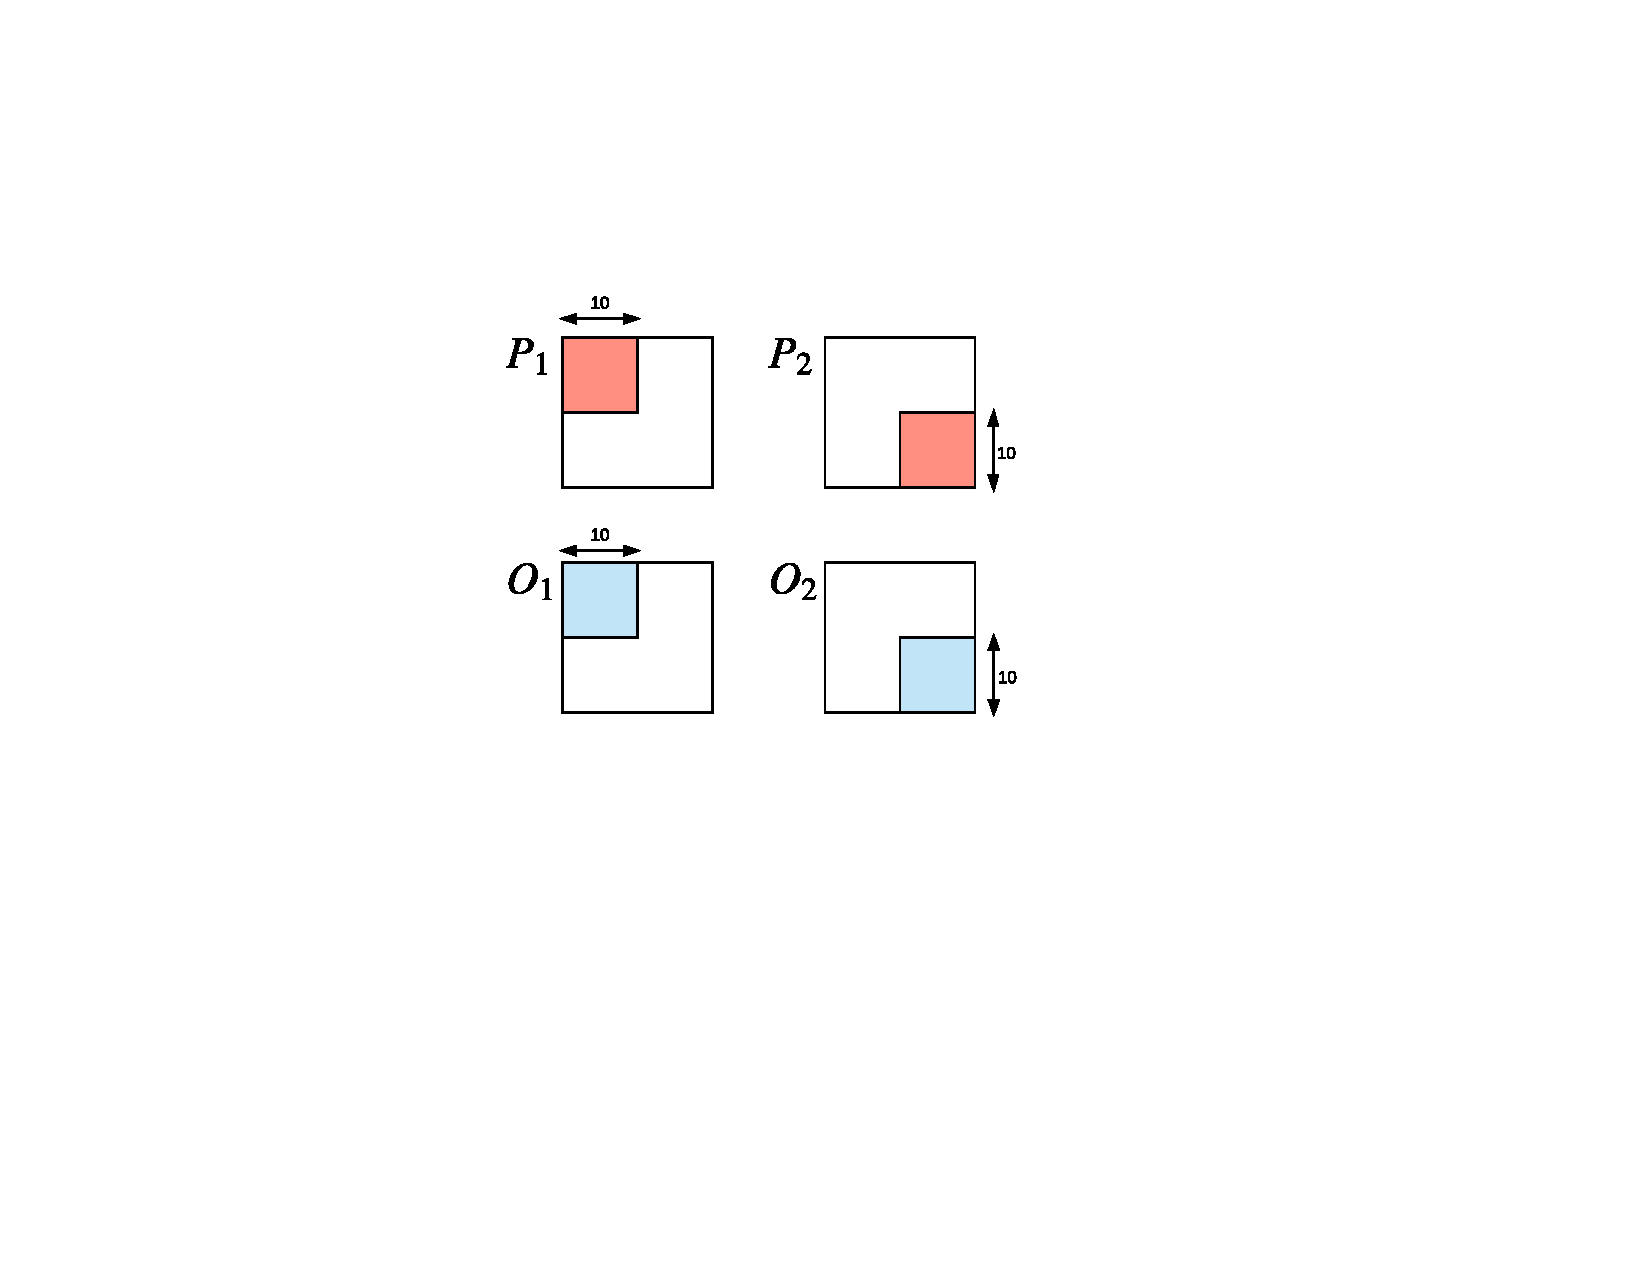
\includegraphics[width=\textwidth]{./img/case1-2}
			\caption{Case 1}
			\label{fig:case1}
		\end{subfigure}
		~ %add desired spacing between images, e. g. ~, \quad, \qquad, \hfill etc. 
		%(or a blank line to force the subFig onto a new line)
		\begin{subfigure}[b]{0.15\textwidth}
			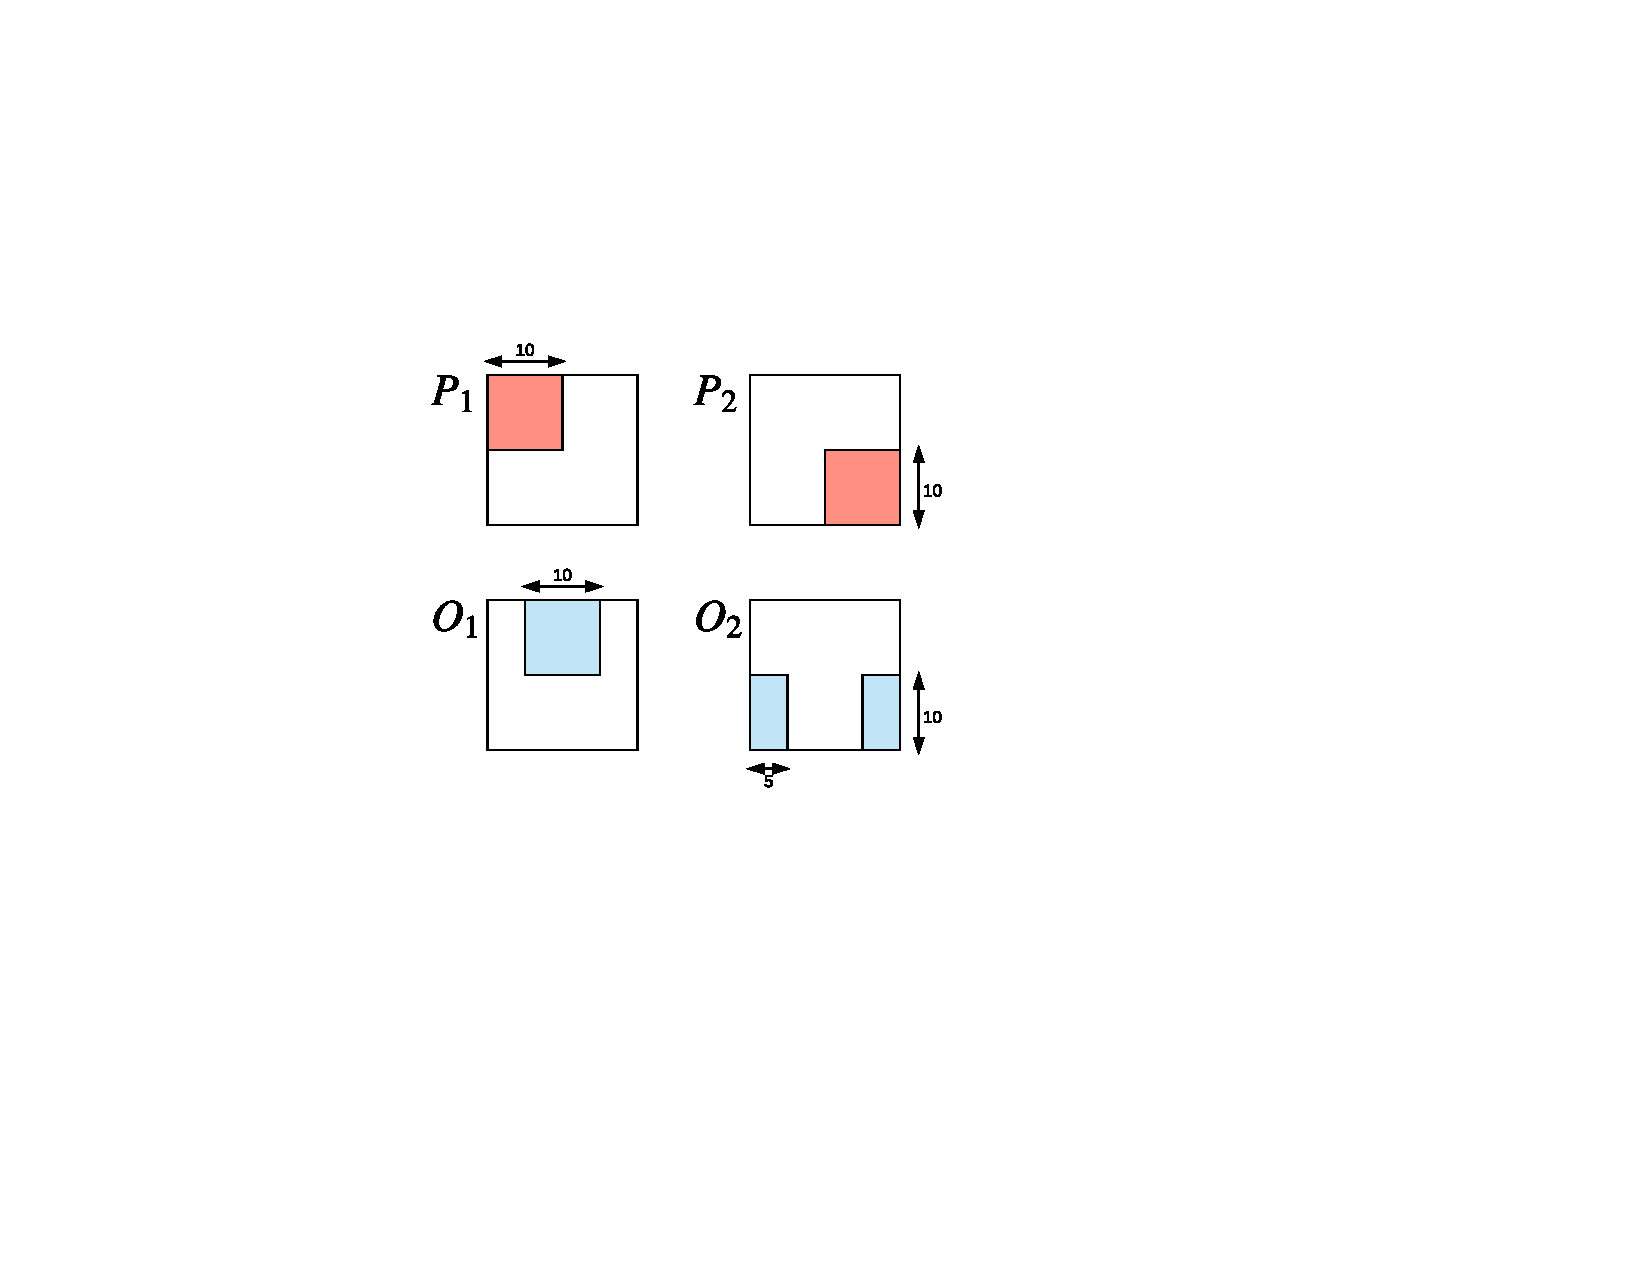
\includegraphics[width=\textwidth]{./img/case2-2}
			\caption{Case 2}
			\label{fig:case2}
		\end{subfigure}
		~ %add desired spacing between images, e. g. ~, \quad, \qquad, \hfill etc. 
		%(or a blank line to force the subFig onto a new line)
		\begin{subfigure}[b]{0.15\textwidth}
			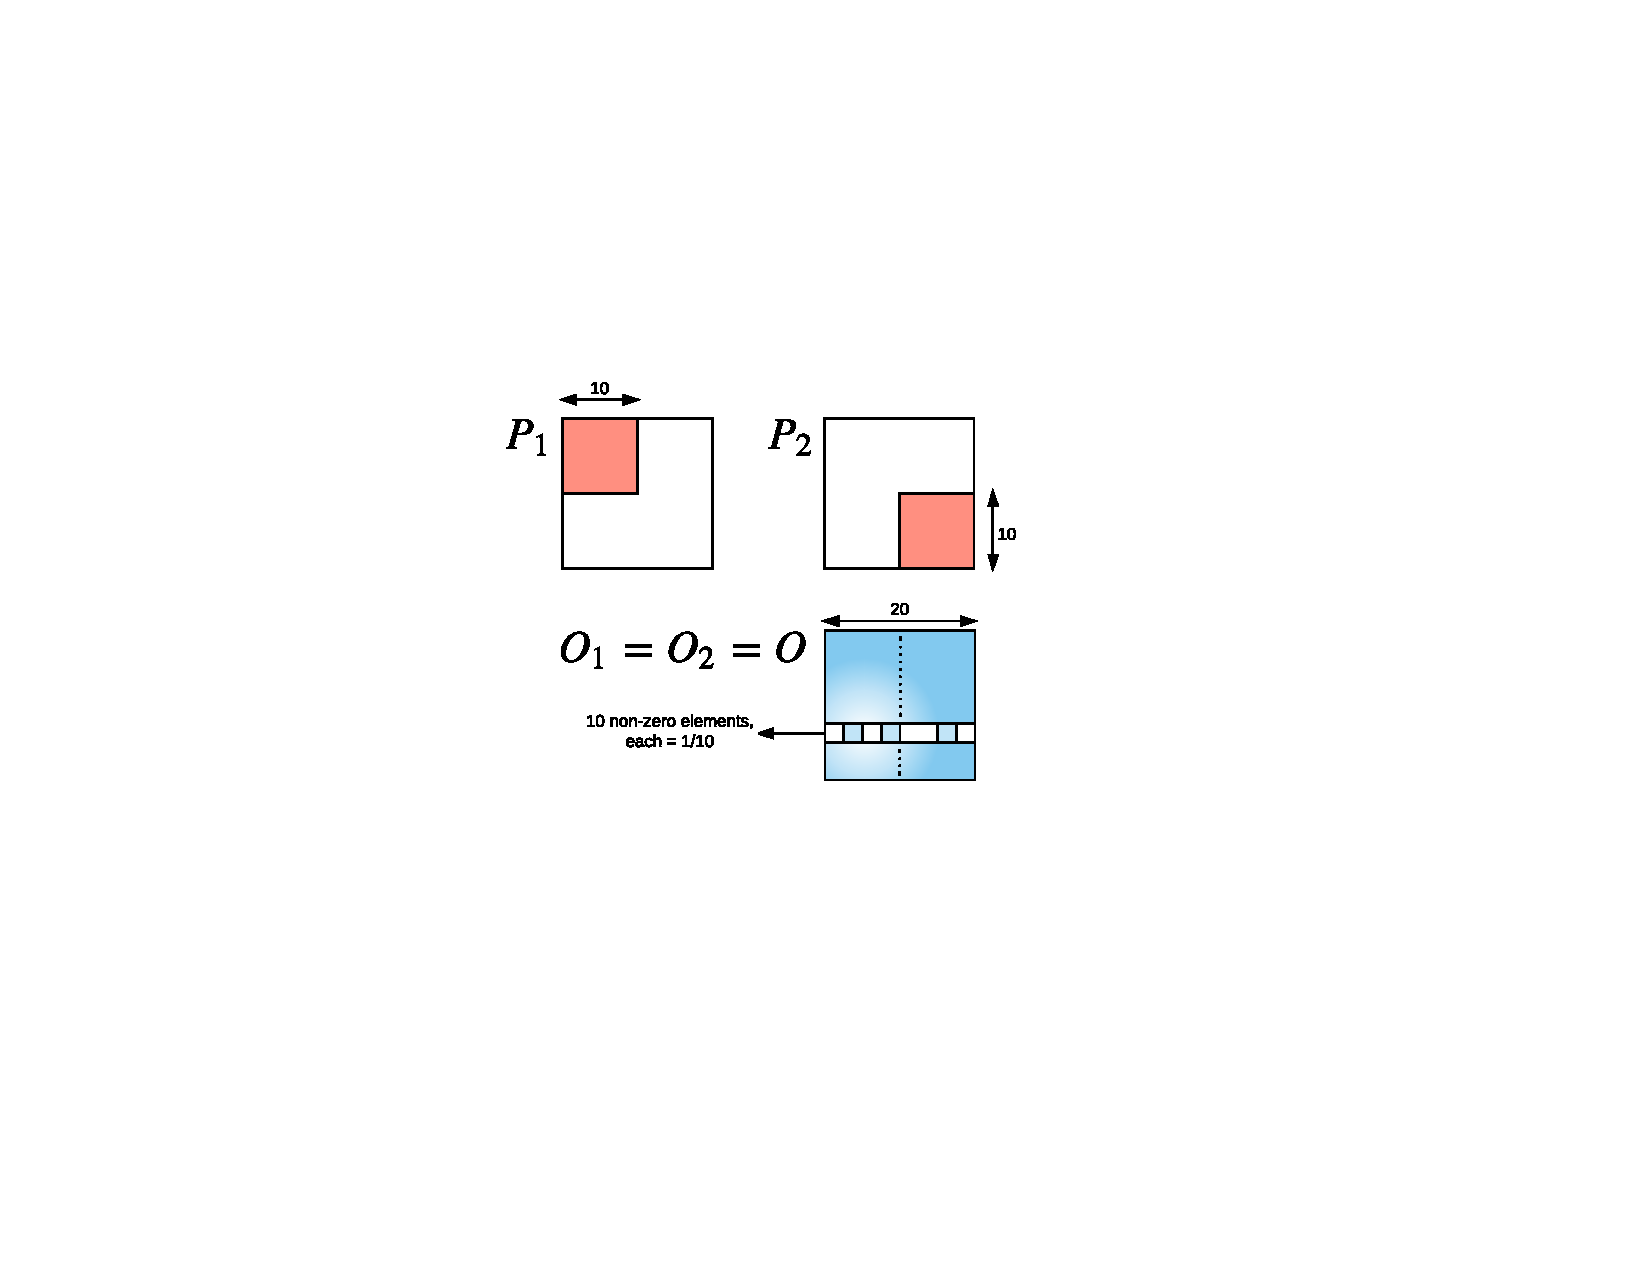
\includegraphics[width=\textwidth]{./img/case3-2}
			\caption{Case 3}
			\label{fig:case3}
		\end{subfigure}
		\caption{Illustration of the disjoint surfing categories for $a = 10$ and $b = 20$.}\label{fig:dsurf}
	\end{figure}
	
	
	\begin{figure}
		\centering
		\begin{subfigure}[b]{0.22\textwidth}
			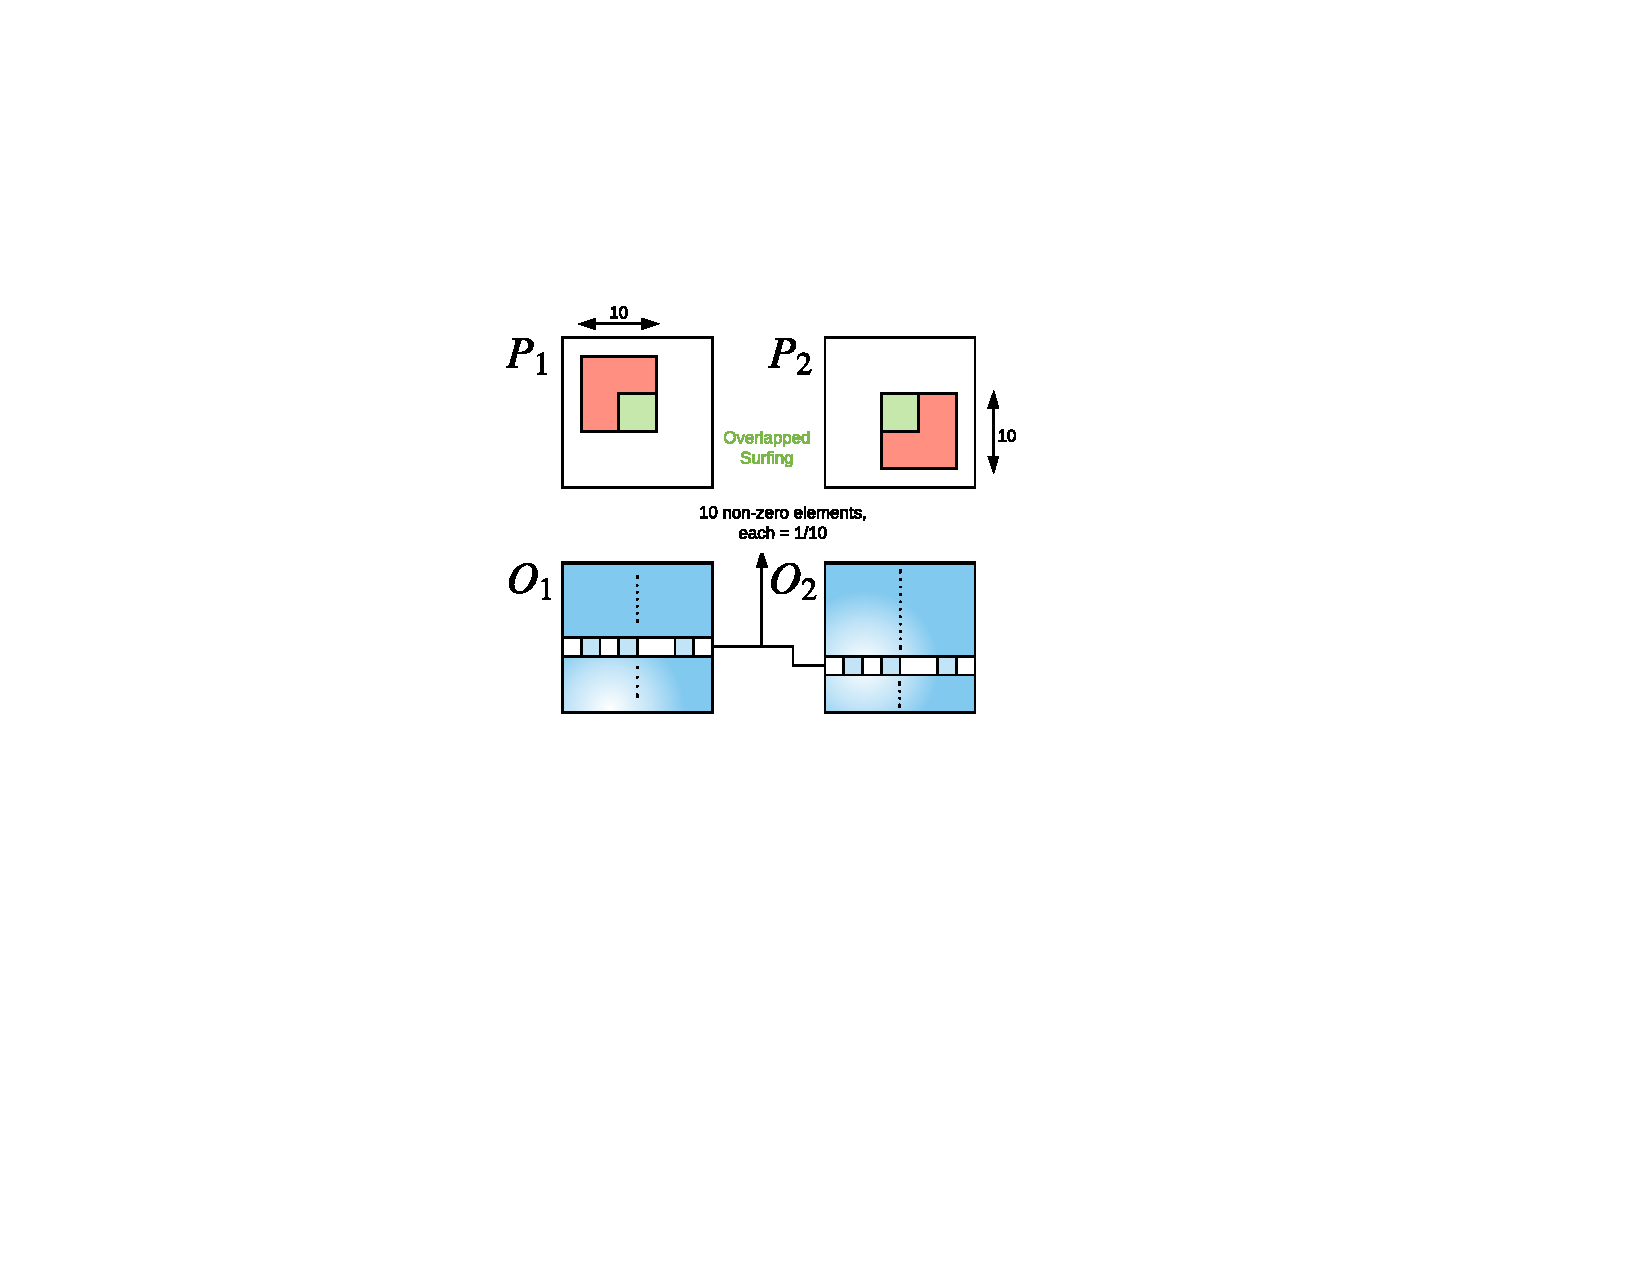
\includegraphics[width=\textwidth]{./img/case4-2}
			\caption{Case 4}
			\label{fig:case4}
		\end{subfigure}
		~ %add desired spacing between images, e. g. ~, \quad, \qquad, \hfill etc. 
		%(or a blank line to force the subFig onto a new line)
		\begin{subfigure}[b]{0.22\textwidth}
			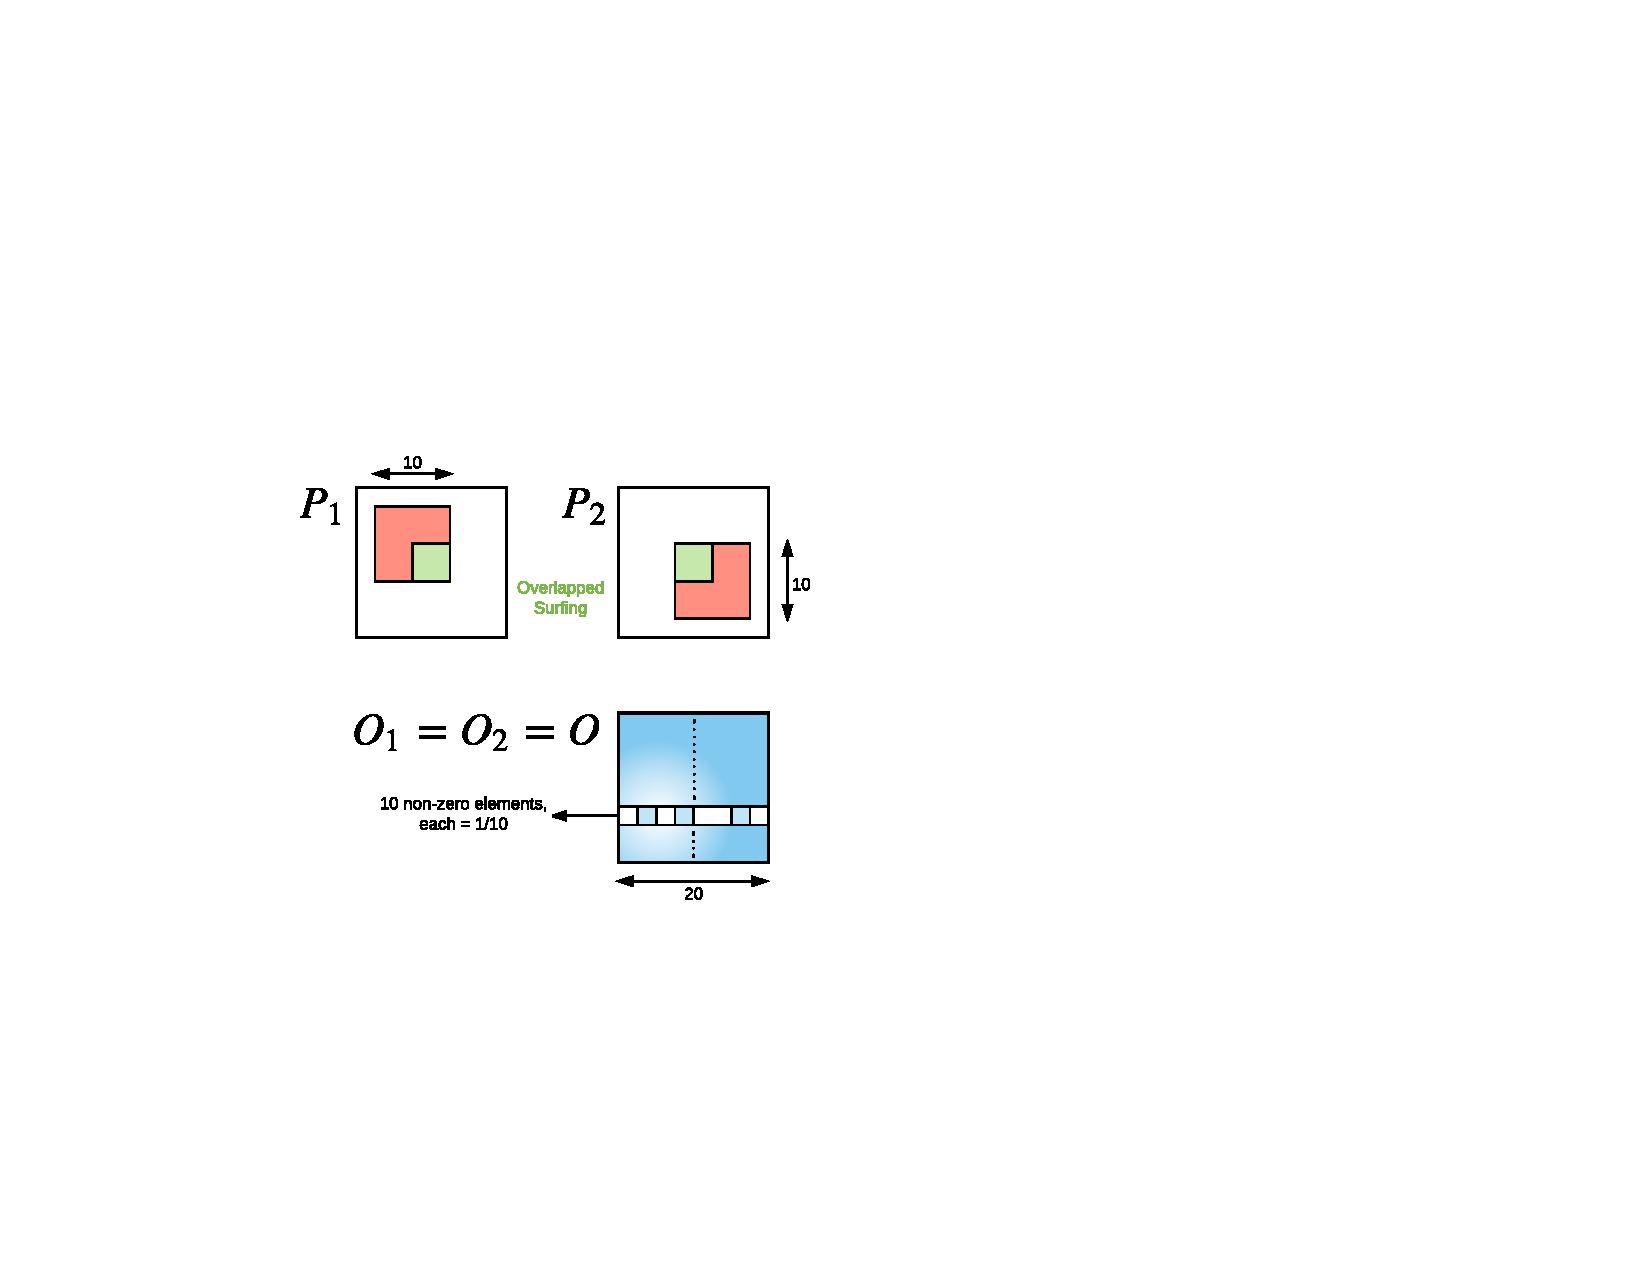
\includegraphics[width=\textwidth]{./img/case5-2}
			\caption{Case 5}
			\label{fig:case5}
		\end{subfigure}
		\caption{Illustration of the overlapped surfing without auxiliary block for $a = 10$ and $b = 20$.}\label{fig:osurf}
	\end{figure}
	
	
	\begin{figure}
		\centering
		\begin{subfigure}[b]{0.22\textwidth}
			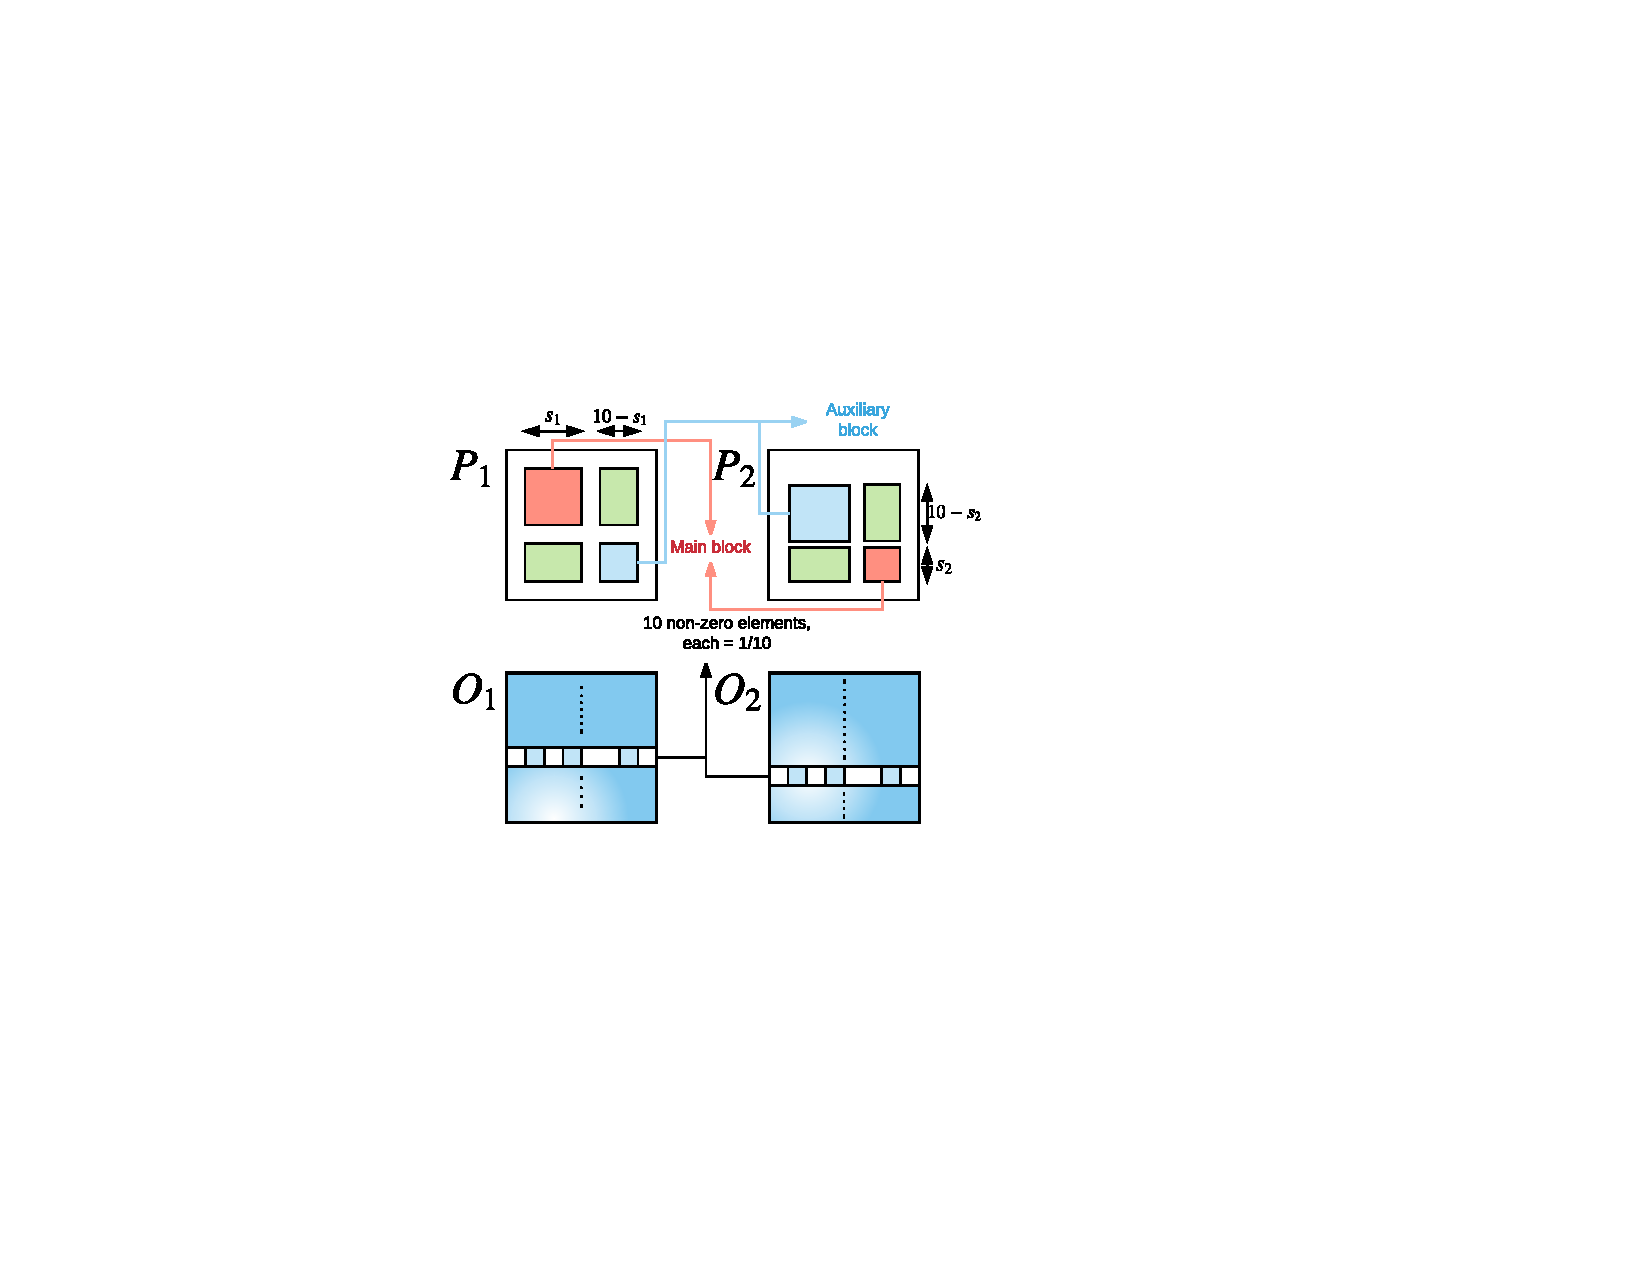
\includegraphics[width=\textwidth]{./img/case6-2}
			\caption{Case 6}
			\label{fig:case6}
		\end{subfigure}
		~ %add desired spacing between images, e. g. ~, \quad, \qquad, \hfill etc. 
		%(or a blank line to force the subFig onto a new line)
		\begin{subfigure}[b]{0.22\textwidth}
			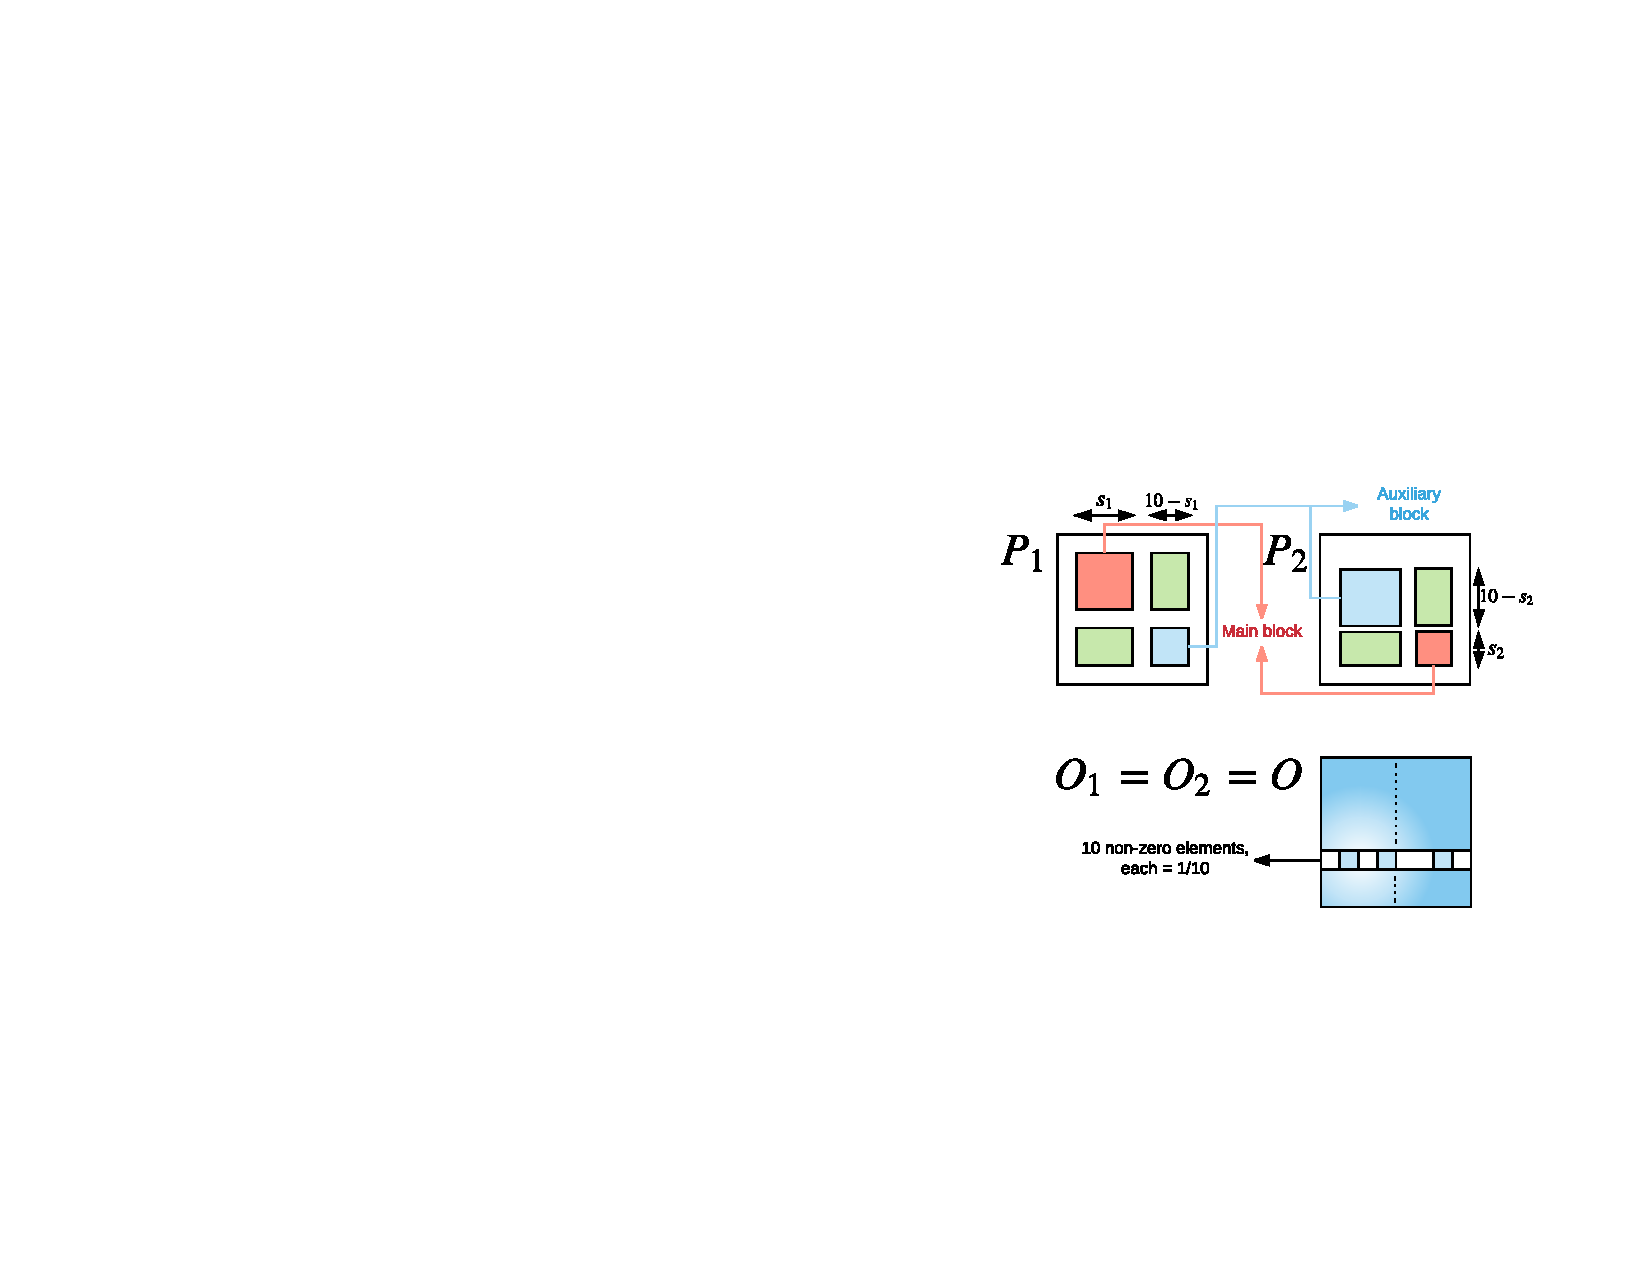
\includegraphics[width=\textwidth]{./img/case7-2}
			\caption{Case 7}
			\label{fig:case7}
		\end{subfigure}
		\caption{Illustration of the overlapped surfing with auxiliary block for $a = 10$ and $b = 20$.}\label{fig:osurfau}
	\end{figure}
	
	{\bf Probability Distributions:}
	\label{subsub:dist}
	Here we explain different distributions used in our synthetic generator:
	\begin{itemize}
		\item {Users shares vector $\aalpha$:} We fix $\aalpha$ to $(.4, .6)$.
		
		\item {Rows of user transition matrix $\A(u)$:} This is a diagonal dominant matrix, meaning that if user $u$ has submitted the current request $v(t)$ it is more probable that he submit the next request. 
		In this way, we capture the fact that because of the episodic nature of the request submission, close-by queries are more probable to come from a same user. 
		This has been exploited in the previous literature \cite{sigcomm}. Note that when instead of matrix $\A$ we only consider the vector $\aalpha$ we may not capture this realistic property of the data.
		For the toy example, we set $\alpha_{ii} = .5 + \frac{1}{2} \text{Uniform}(0,1)$ and $\forall i \neq j: \alpha_{ij} \propto (1 - \alpha_{ii}) \text{Uniform}(0,1)$
		
		\item {Rows of output matrix $\O_u(w)$:} As mentioned before, each row $\O_u(w)$ has $a$ non-zero elements with each with probability $1/a$.
		
		\item {Rows of page transition matrix $\P_u(w)$:} In a nutshell, we discretize a continuous Beta distribution with different parameters for each block and normalize the final vector.
		The distribution that we use for the (main) support is Beta(3+$\epsilon$,1+$\delta$) where $\epsilon$ and $\delta$ are random numbers from $[-1, 1]$. 
		For the distribution on the auxiliary support of the cases 6 and 7 above, we use Beta(2+$\epsilon$,2+$\delta$).
	\end{itemize}
	
	
	
	{\bf Discussion:}
	Table \ref{tab:as} shows the error of our method for all 7 cases of Section \ref{subsub:sparsity} for $a = 10$. 
	%Note that we report the result for both RNN and its variant LSTM. 
	
	\begin{table}
		\scriptsize  
		\centering
		\begin{tabular}{|c|c|c|c|c|c|c|c|c|}
			\hline
			\multicolumn{2}{|c|}{\bf \footnotesize Cases} & {\bf \footnotesize  1} & {\bf \footnotesize  2} & {\bf \footnotesize  3} & {\bf \footnotesize  4} & {\bf \footnotesize  5} & {\bf \footnotesize 6} & {\bf \footnotesize  7}  \\ 
			\hline  
			\multirow{2}{*}{$\aalpha$} & {\footnotesize  Mean} 	&  1 	& 1		&  .63 &  .70 & .62 &  .74& .65 \\ \cline{2-9}
			                           & {\footnotesize  Std} 	&  0 	& 0 	&  .02 &  .02 & .02 &  .05& .04 \\ \hline 
			\hline  
			\multirow{2}{*}{$A$}       & {\footnotesize  Mean} 	&  1 	& 1		&  .77 & .69 &  .67 & .82 & .78 \\ \cline{2-9}
			                           & {\footnotesize  Std} 	&  0 	& 0		&  .10 & .09 &  .08 & .09 & .16 \\ \hline 
		\end{tabular}
		\caption{Deinterleaving accuracy of= LSTM for different cases of the synthetic example when user transitions are determine by either of $\aalpha = [.4, .6]$ or random diagonally dominant $\A$.}
		\label{tab:as}
	\end{table}
	
	Each row is the average result for five instantiation of the model parameters $\O_u$ and $\P_u$. 
	The error of each instantiation (each row) is an average of 100 experiments. 
	Note that case 1 and 2 are trivial cases when both $\P$s and $\O$s are disjoint and LSTM perfectly dis-interleave. 
	Interestingly, performance in case 3 is much worse than cases 1 and 2, which confirms that in our model having disjoint output matrices is more important than disjoint surfing pattern. 
	Intuitively, this makes sense because the final request comes from the output matrices and if we have personalized outputs the deinterleaving should be easier. 
	Interestingly, beyond the trivial cases 1 and 2, case 6 has the best accuracy, probably because of personalized outputs and more complicated $\P_u$ for each user (composed of main and auxiliary block) makes the whole problem more separable. 
	
	%	This is by far better than what we have or even the literature of dis-interleaving has. 
	%	For (.4, .6) user share of requests, previous results (even in simple Markov chain interleaving not HsMM) are around at most .65 but here on the last experiment, we get about .78 accuracy. 
	%	Also, we are still measuring accuracy as the exact match between the inferred user and true users for all pages, which as we talked last time is a harsh criterion. 
	%	Vinod suggested that we should measure the accuracy only for the "popular enough" pages (We would appreciate if you can elaborate on this.)  
	
%	Since RNN and LSTM performances are very close and LSTM is more computationally demanding, in the following experiments we will only use RNN method. 
%	Note that when we use $\A$ instead of $\aalpha$ the error is smaller. 
%	This can be explained by the fact that with the diagonally dominated user transition matrix $\A$ neighbor requests in the resolver are more probable coming from a same user and this extra structure will help the algorithm to deinterleave more efficiently. 
%	
%	%	\subsubsection{Comparison with Viterbi Coding}
%	
%	
%	\subsubsection{Scalability}
%	In this set of synthetic experiment we increase the number of users and number of webpages report the performance of RNN-based deinterleaving methods. 
%
%	{\bf Scaling Users:}
%	\label{subsub:scalseusr}
%	In this set of experiments we increase the number of users and evaluate the performance of our RNN based method while changing the number of layers and hidden units of RNN. 
%	It is expected that adding more users makes the deinterleaving harder and therefore the error will increase. 
%	We perform two extreme experiments using each $\aalpha$ and $\A$ to control the user transition dynamics: 
%	
%	\begin{itemize}
%		\item User transition with $\aalpha$:
%		\begin{itemize}
%			\item $\aalpha$ is uniform over the users, i.e., $\alpha_i = \frac{1}{m}$. In this case, we expect deinterleaving to be very hard because there is no distinction between request generation rate of users. 
%			%			\item $\aalpha_i$ decreases geometrically in $i$, i.e., $\alpha_i = (1 - 2^{-m})^{-1} \times .5^i $
%		\end{itemize}
%		\item User transition with $\A$:
%		\begin{itemize}
%			%			\item $\alpha_{ii} = .5 + \frac{1}{2} \text{Uniform}(0,1)$ and $\forall i \neq j: \alpha_{ij} = (1 - \alpha_{ii}) \frac{1}{m - 1}$
%			\item $\alpha_{ii} = .5 + \frac{1}{2} \text{Uniform}(0,1)$ and $\alpha_{ij} = 
%			\begin{cases}
%			(1 - \alpha_{ii}) (1 - 2^{-m+1})^{-1} .5^j,     \quad j < i \\
%			(1 - \alpha_{ii}) (1 - 2^{-m+1})^{-1} .5^{j-1}, \quad j > i
%			\end{cases} 
%			$. 
%			Here, we have two properties that we hope to make deinterleaving easier. 
%			First, $\A$ is diagonally dominant which makes close-by queries more probable to come from same users. 
%			Also, the overall probability of picking users as active is non-uniform. 
%		\end{itemize}
%	\end{itemize} 
%	We perform experiment on $2, 5,$ and $10$ users and generate the synthetic data using the Case 6 of Section \ref{subsub:sparsity}. 
%	Maximum number of requests per page is limited to 5 and total number of pages $n$ is $1000$ while the support size of rows of matrices $a$ is $100$. 
%
%	
%%	\begin{figure}
%%		\centering
%%		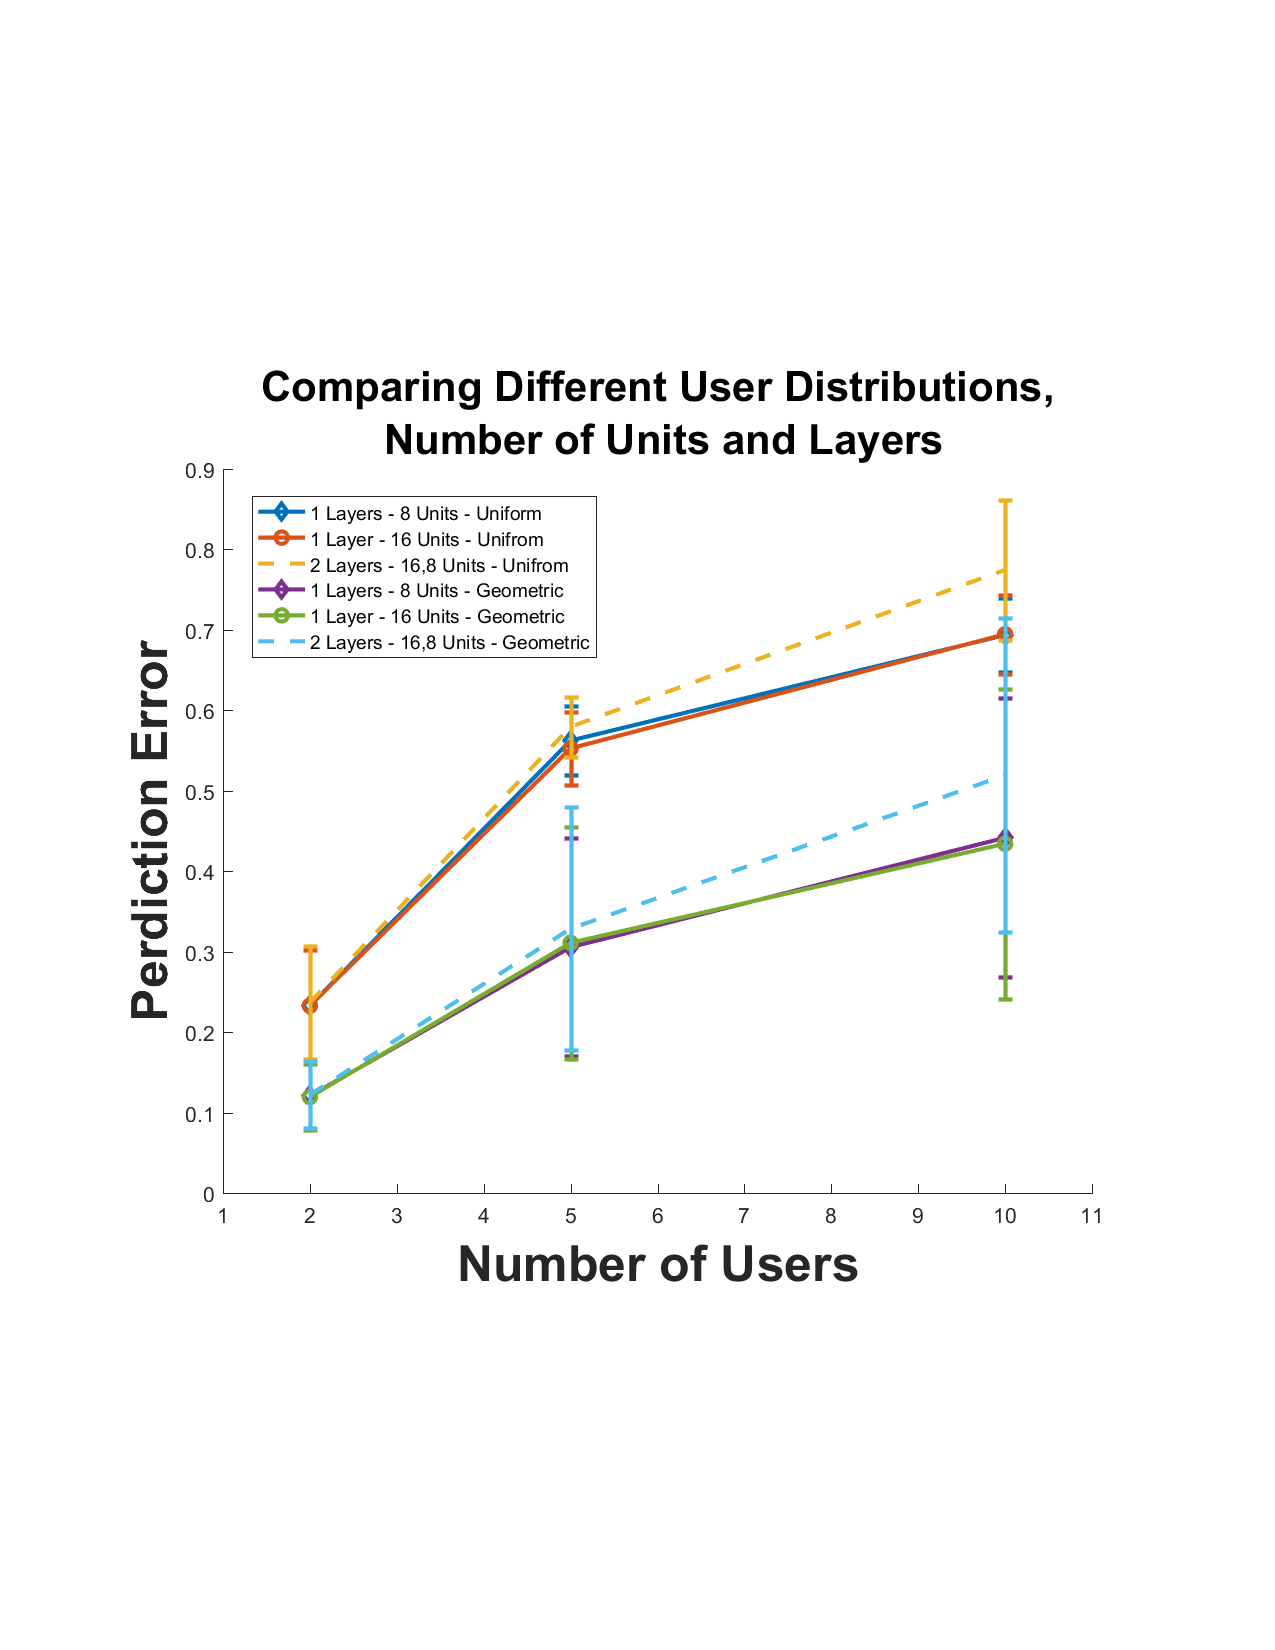
\includegraphics[width=.7\textwidth]{./img/users4}
%%		\caption{Comparing error for different user distributions, number of hidden layers and units.}
%%		\label{fig:user}
%%	\end{figure}
%	Fig \ref{fig:user} illustrates that deinterleaving becomes harder as we increase the number of users. 
%	But for the more realistic setup of user transition with matrix A even for 10 users we can reach 50\% accuracy.
%	Note that increasing the number of units is not helping the performance and increasing the layers overfits the data. 
%	
%	
%	{\bf Scaling Pages:}
%%	In this synthetic experiment we test the performance of our algorithm for two users with $\aalpha = [ .4, .6 ]$ while we increase the total number of pages $b$ linearly while keeping the support of each row of matrices as $a = n / 10$. 
%	In this synthetic experiment we test the performance of our algorithm for two users with matrix $\A$ generated as Section \ref{subsub:scalseusr} while we increase the total number of pages $b$ exponentially while keeping the support of each row of matrices as $a = n / 10$.
%	Maximum number of requests per page is limited to 5 and total number of pages $b$ is from the set $\{ 10^2, 10^3, 10^4, 10^5 \}$.
%	Based on the results of the user scalability experiment, we pick single layer RNN with 8 units. 
%	Fig \ref{fig:incpages} shows that as we increase the number of pages denterleaving becomes harder. 
%%	\begin{figure}
%%		\centering
%%		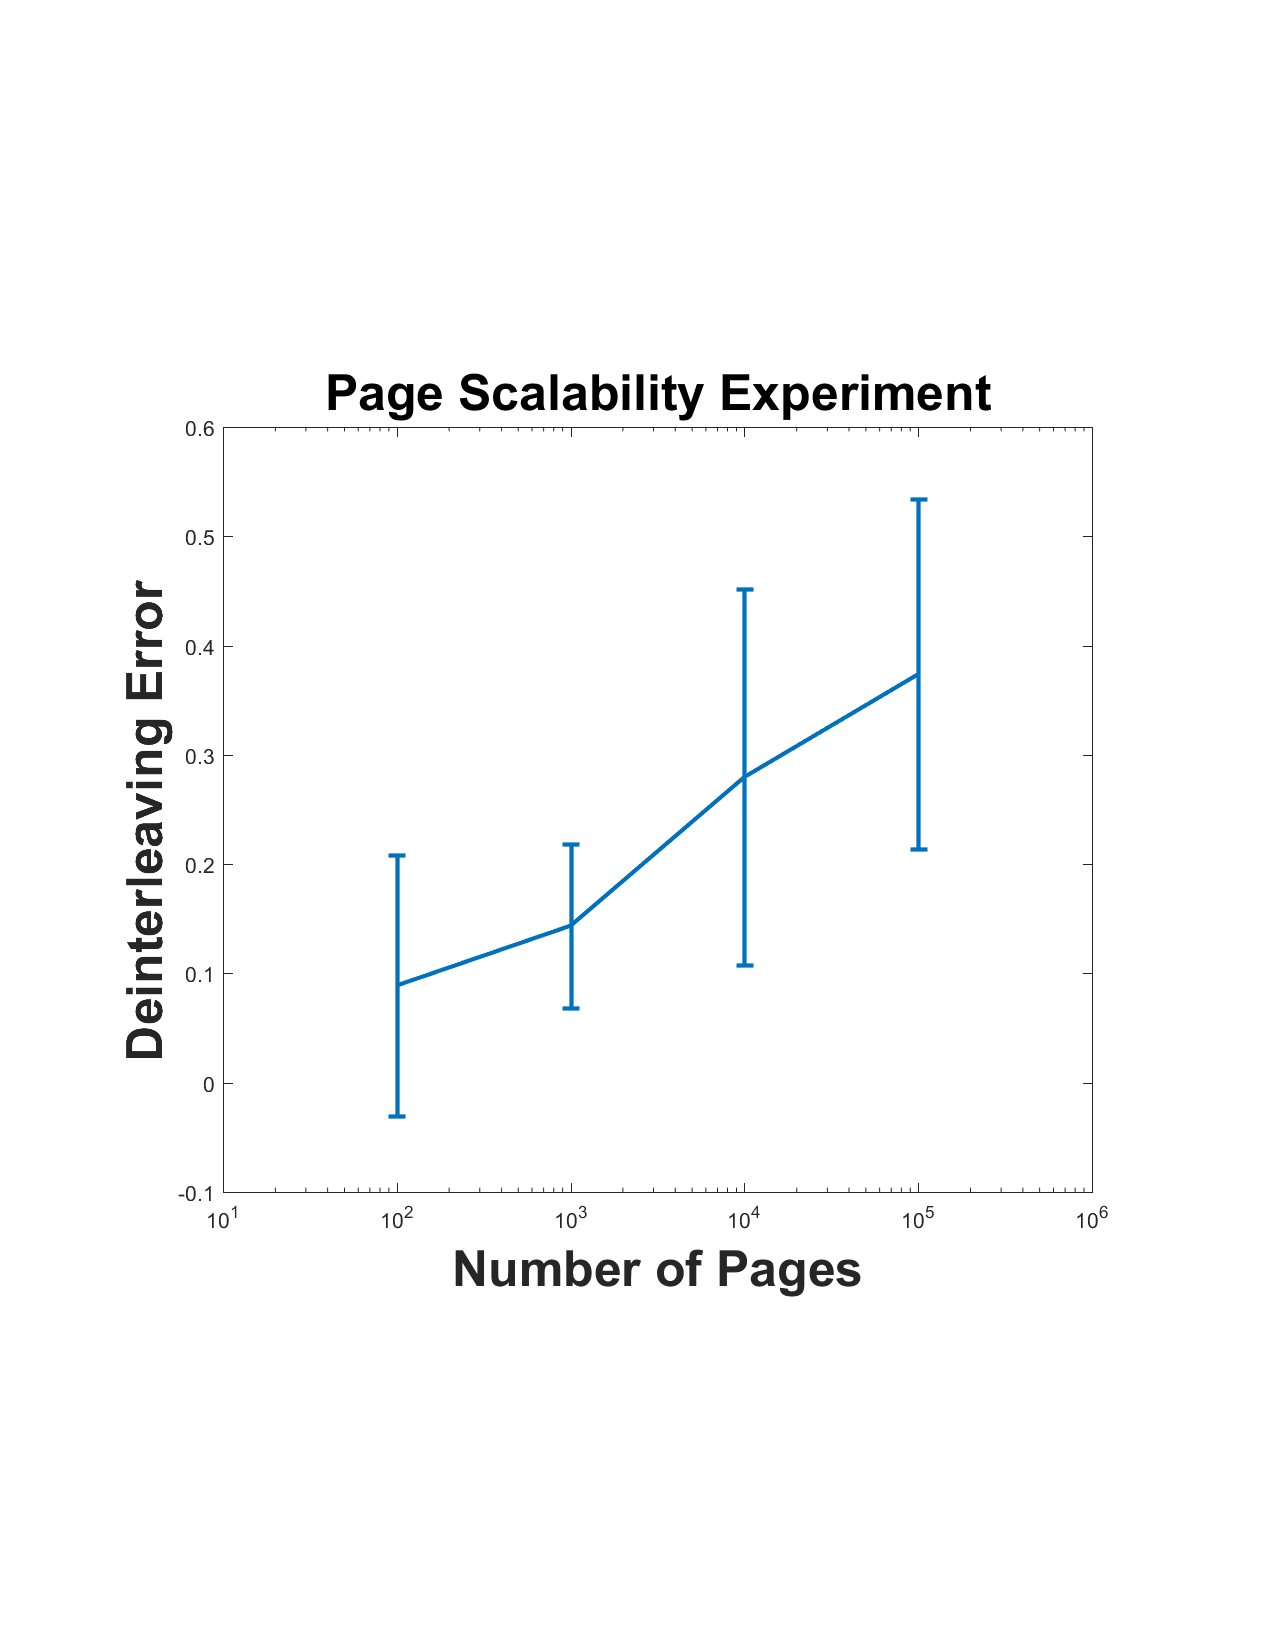
\includegraphics[width=.7\textwidth]{./img/incpages2}
%%		\caption{Scaling pages experiments.} 
%%		\label{fig:incpages}
%%	\end{figure}
%%	
%	\begin{figure}
%	\centering
%	\begin{subfigure}[b]{0.45\textwidth}
%		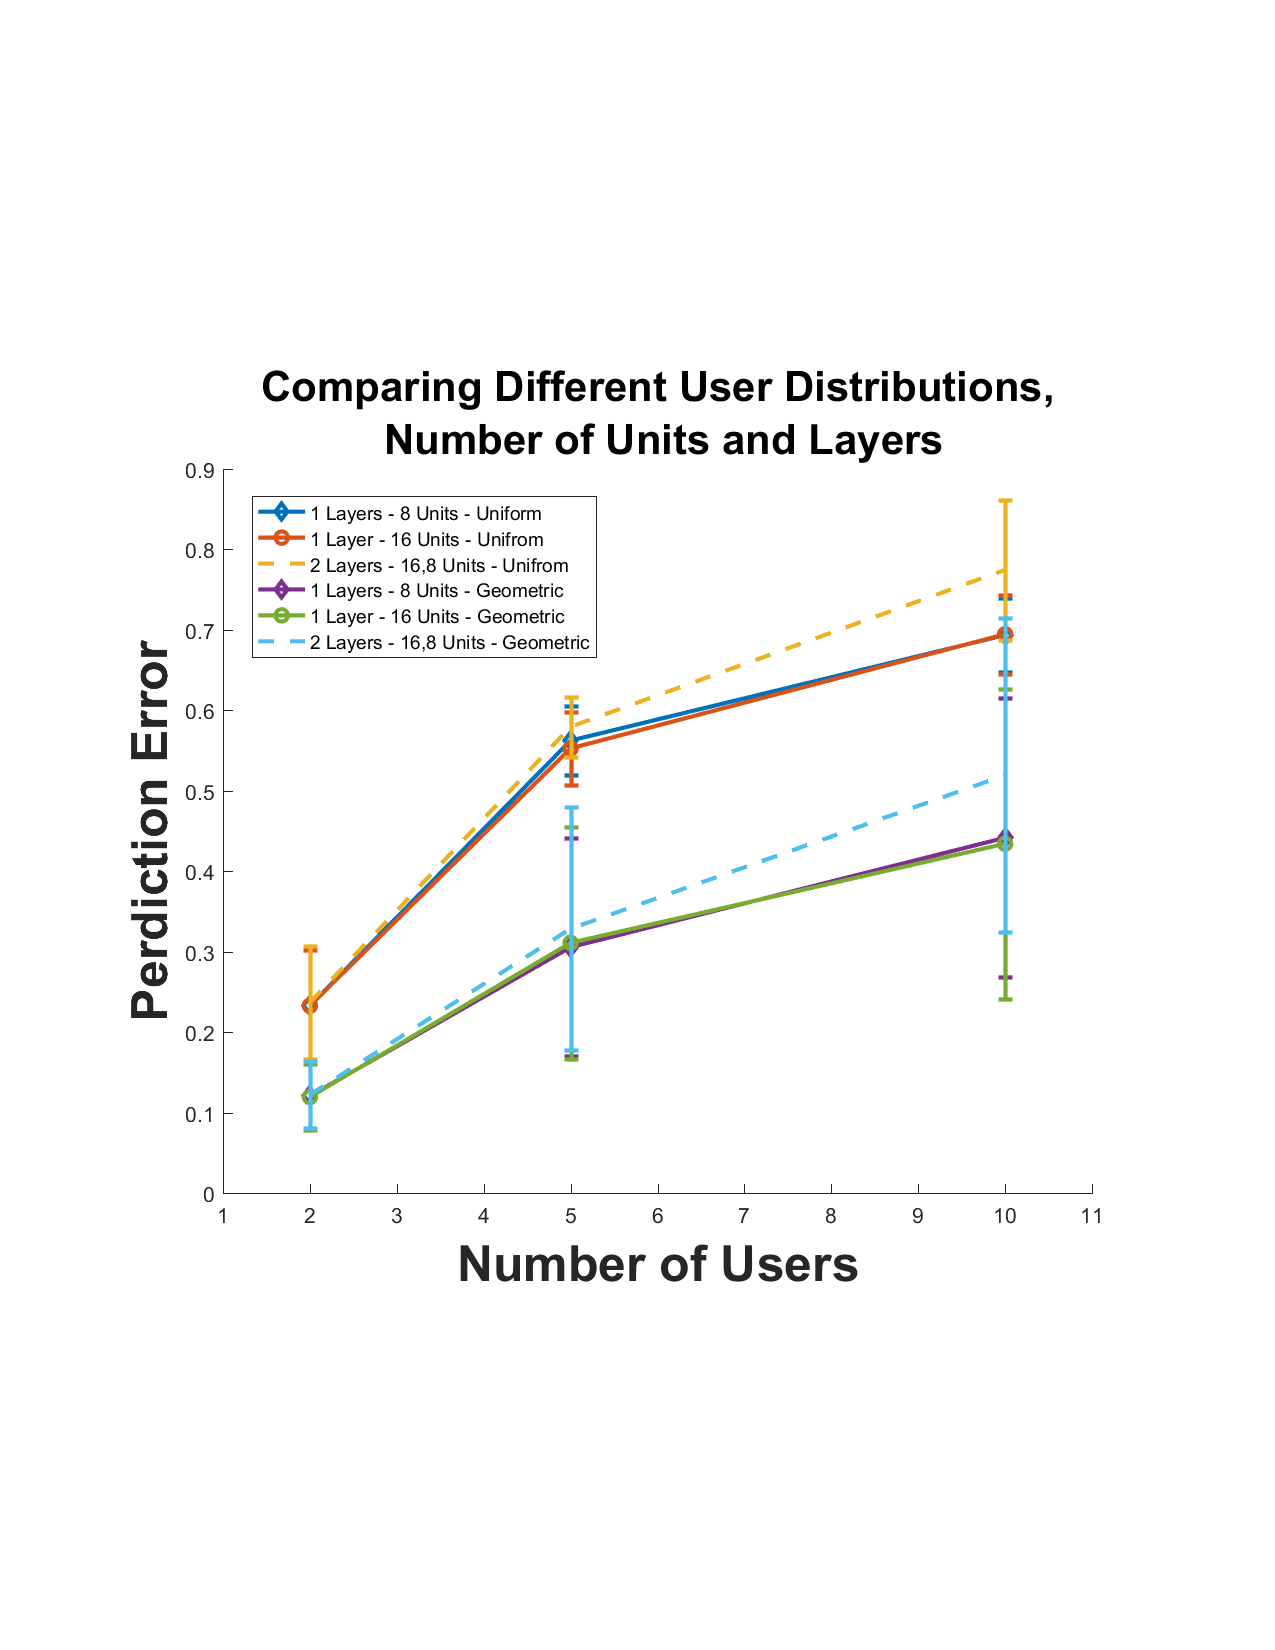
\includegraphics[width=\textwidth]{./img/users4}
%		\caption{Increasing number of users.}
%		\label{fig:user}
%	\end{subfigure}
%	~ %add desired spacing between images, e. g. ~, \quad, \qquad, \hfill etc. 
%	%(or a blank line to force the subFig onto a new line)
%	\begin{subfigure}[b]{0.45\textwidth}
%		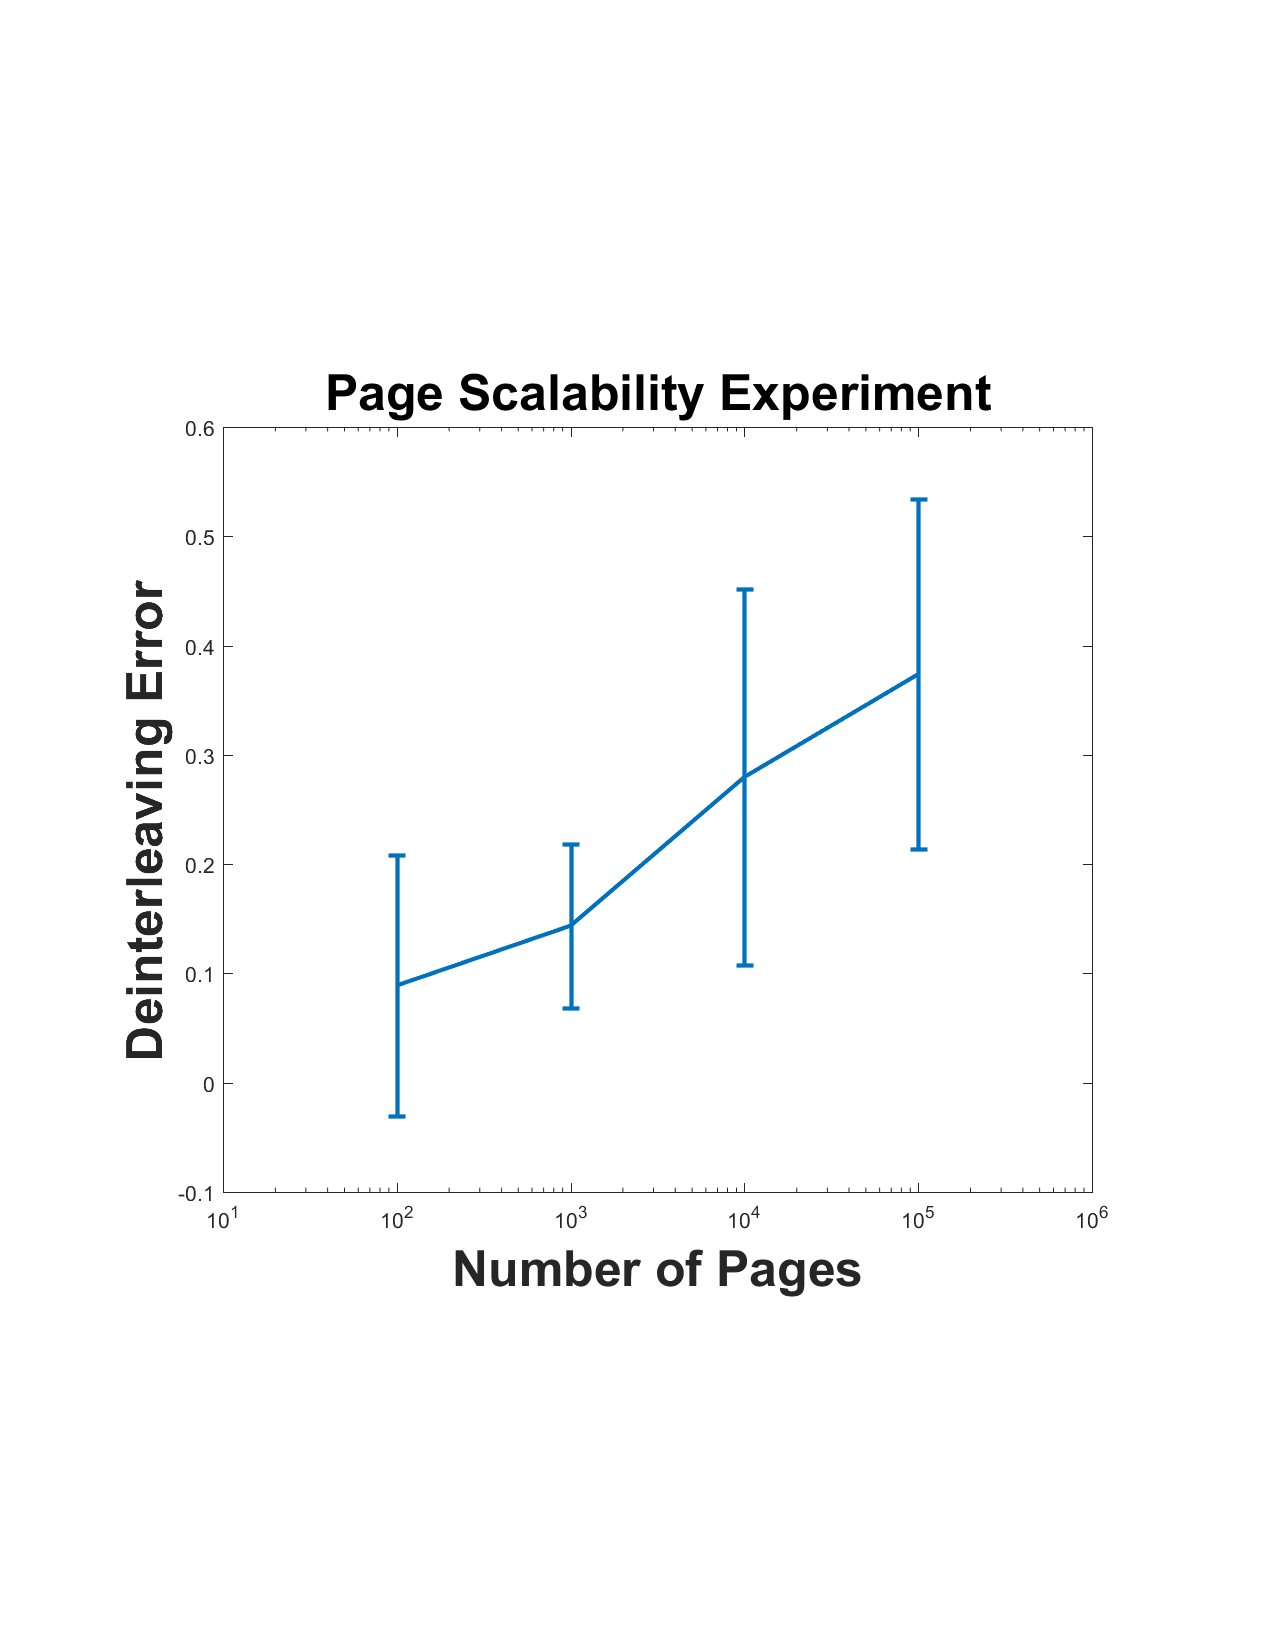
\includegraphics[width=\textwidth]{./img/incpages2}
%		\caption{Increasing number of pages.}
%		\label{fig:incpages}
%	\end{subfigure}
%	\caption{Scalability Experiment.}%\label{fig:osurfau}
%	\end{figure}
%	
%	\subsection{Real Data}
%	
%	
	
	
	
	%	Following are the results of the experiment in two separate setup. 
	%	First we assume that we know the parameters mentioned in Table \ref{tab:toy} and run the Viterbi algorithm and compute the accuracy for user, page, and state recovery.
	%	Next, we learn the parameters from the sequences using the Baum-Welch algorithm, then use the same sequence for Viterbi decoding and compute the accuracies. 
	%	
	%	\begin{figure}
	%		\centering
	%		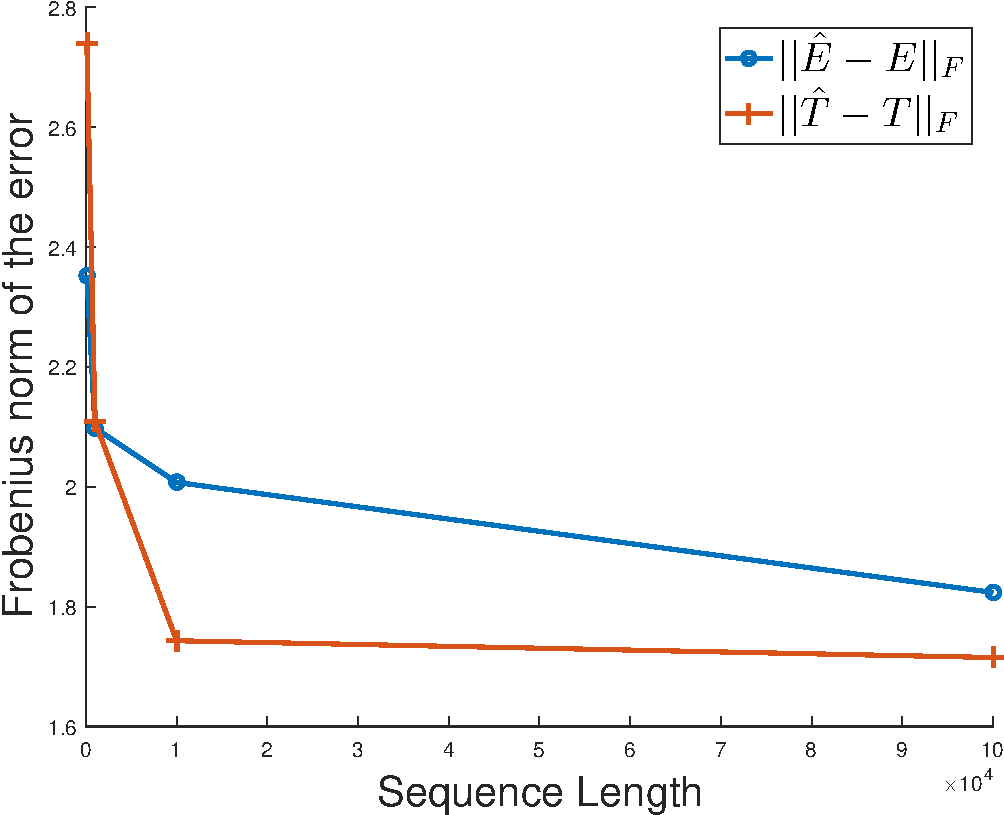
\includegraphics[scale=.4]{./img/frob-cropped}
	%		\caption{Error in learning transition matrix $T$ and emission matrix $E$ after 500 iterations of Baum-Welch algorithm (algorithm stops if the change in the log-likelihood of the observed sequence is less than 1e-6).}
	%		\label{fig:frob}
	%	\end{figure}	
	%	\begin{figure}
	%		\centering
	%		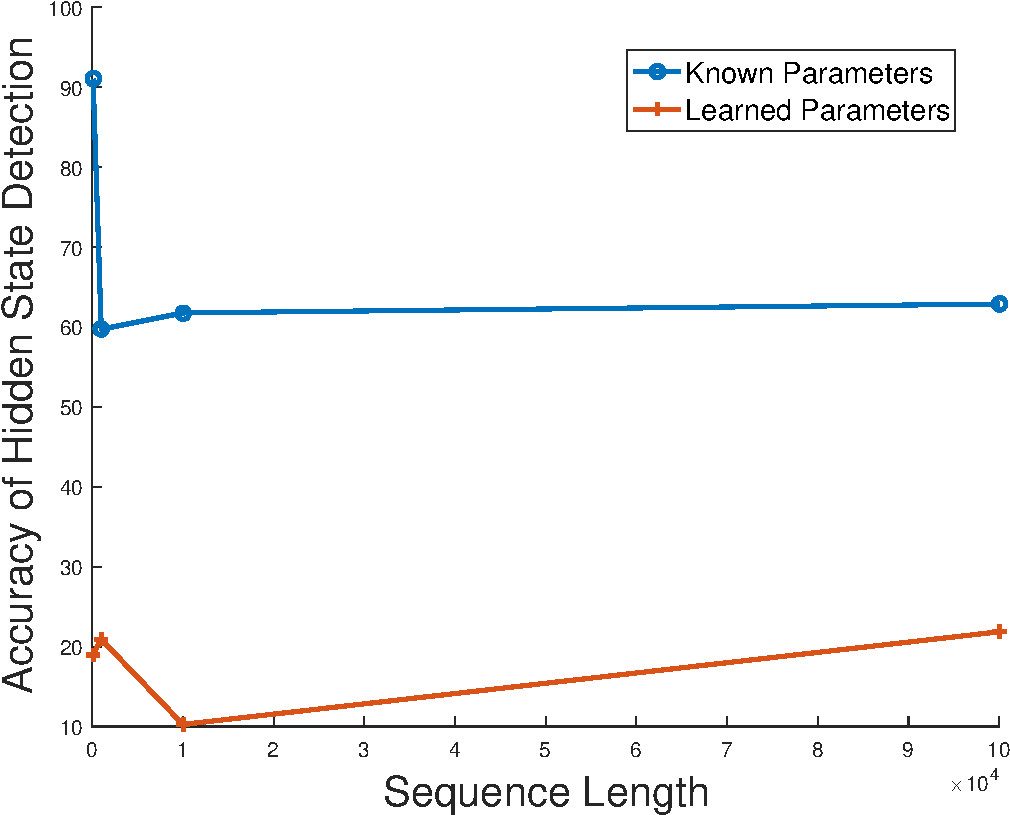
\includegraphics[scale=.4]{./img/states-cropped}
	%		\caption{Accuracy of hidden state detection using Viterbi for known and learned parameter. Obviously we do better when the parameters are known. Also for the unknown parameter as the number of samples increases, we learn the parameters more accurately \ref{fig:frob} which also improves Viterbi coding. The drop from 1000 to 10000 may be attributed to the fact that BW algorithm does not converge after 500 iterations when we go beyond 1000.}
	%		\label{fig:states}
	%	\end{figure}
	%	
	%	\begin{figure}
	%		\centering
	%		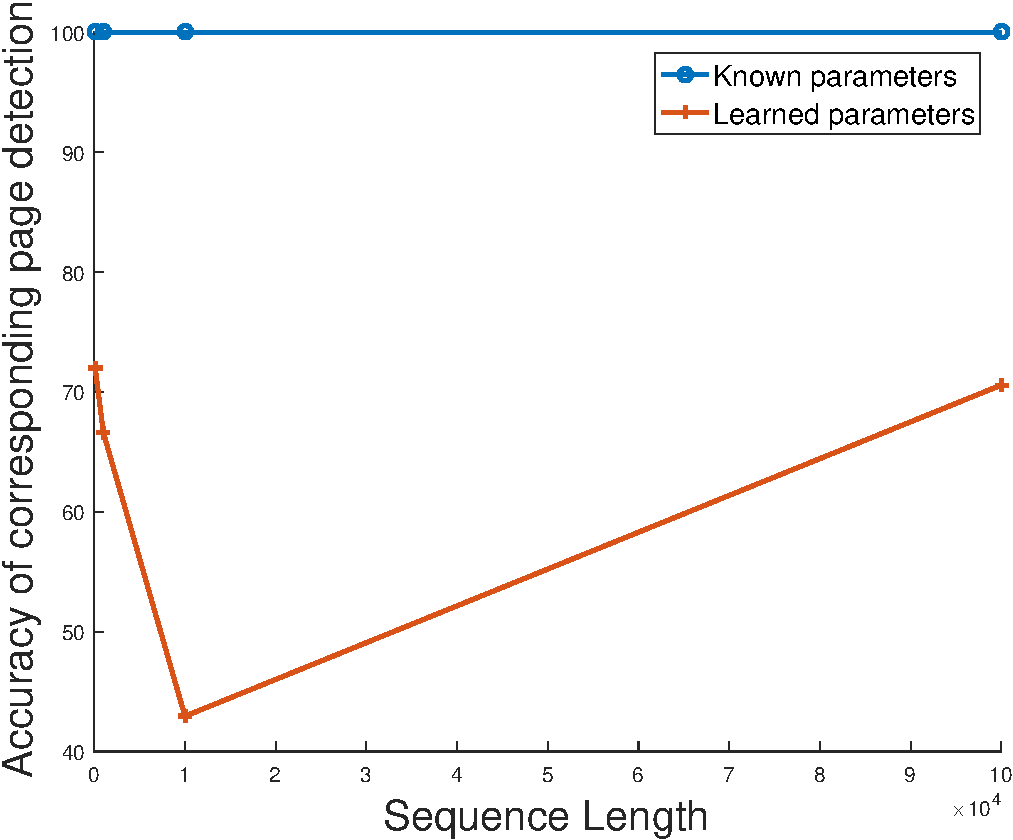
\includegraphics[scale=.4]{./img/pages-cropped}
	%		\caption{Accuracy of hidden page detection using Viterbi for known and learned parameter. We do prefect when the parameters are known. Also for the unknown parameter as the number of samples increases, we learn the parameters more accurately \ref{fig:frob} which also improves Viterbi coding. The drop from 1000 to 10000 may be attributed to the fact that BW algorithm does not converge after 500 iterations when we go beyond 1000. I think here we do better in comparison to user detection, because observation (visible sequence) depends completely on pages not users.}
	%		\label{fig:pages}
	%	\end{figure}
	%	
	%	\begin{figure}
	%		\centering
	%		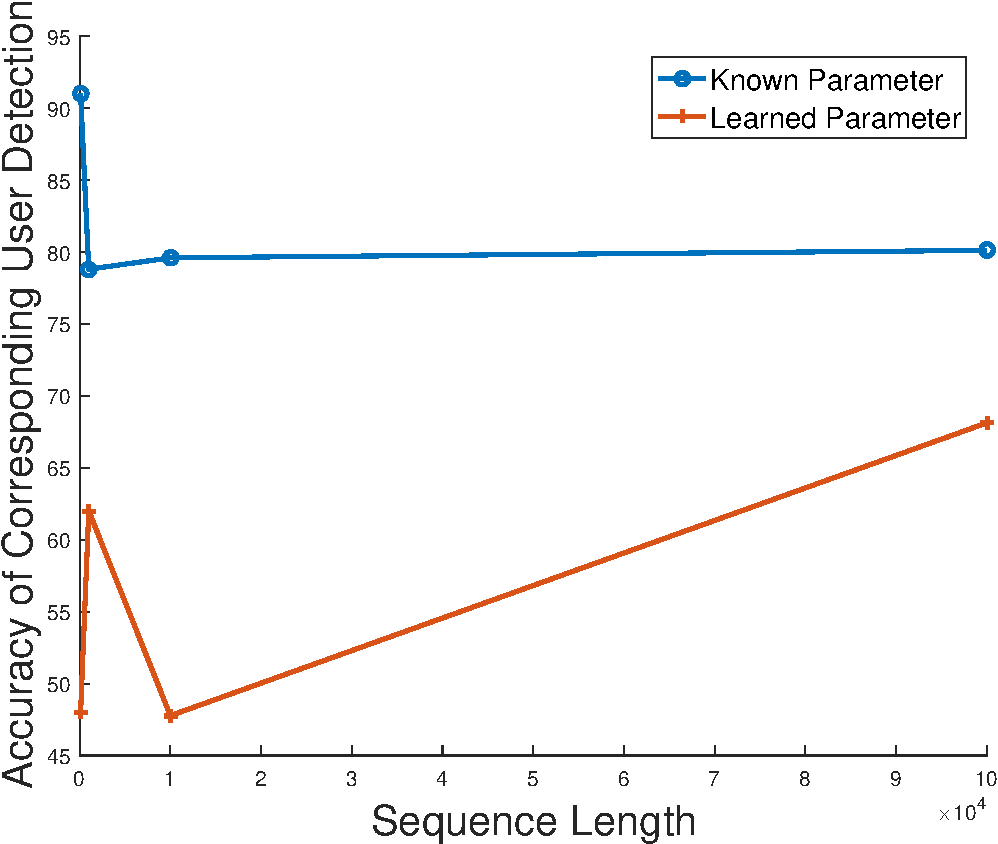
\includegraphics[scale=.5]{./img/users-cropped}
	%		\caption{Accuracy of hidden user detection (dis-interleaving solution) using Viterbi for known and learned parameter. We do around 80 percent with known parameters. Also for the unknown parameter as the number of samples increases, we learn the parameters more accurately \ref{fig:frob} which also improves Viterbi coding. The drop from 1000 to 10000 may be attributed to the fact that BW algorithm does not converge after 500 iterations when we go beyond 1000. I think as the interleaving paper mentioned, if we go from imbalanced $\aalpha = [0.2, 0.8]$ to more uniform $\aalpha$ accuracy drops.}
	%		\label{fig:users}
	%	\end{figure}
	%	
	
	%		
	%	Table \ref{tab:as} summarizes all of the assumptions.
	%	In the following we provide some details. 
	%	\begin{table}
	%		\centering
	%		\begin{tabular}{|c|l|}
	%			\hline
	%			Parameter & Value \\ 
	%			\hline  
	%			$m$ & 2 users \\ \hline
	%			$n$ & 20 pages \\ \hline
	%			$q$ & 1 request per page\\ \hline 
	%			$s$ & 3200 stats for the HMM\\ \hline 
	%			$t$ & 5000 sequence length of HMM (size of the resolver queue).\\ \hline 
	%			\hline 
	%			$\aalpha$ & The user's query generation probability is fixed to $[0.3, 0.7]$. \\ \hline 
	%			$\P_u \in \reals^{n \times n}$ & Entries drawn uniformly at random. \\ \hline 
	%			$p_w(d) \in \reals$ & Uniformly distributed, $d\sim U(1,2)$. \\ \hline 
	%			$\o_w(r) \in \reals^n$ & Drawn uniformly at random on all possible pages (domain names). \\ \hline 
	%		\end{tabular}
	%		\caption{Summary of the experiment setup.}
	%		\label{tab:as}
	%	\end{table}
	
	%	\noindent{\bf Generate Page Transition Matrix:}
	%	For each user we first generate a page transition matrix $\P_u$ completely at random. 
	%	
	%	\noindent{\bf Generate Duration Probability Distribution:}
	%	We assume that the number of requests per page is a uniform random variable over $[1, \texttt{NUM\_REQ}]$ interval.
	%	
	%	\noindent{\bf Generate HMM State Transition Matrix:}
	%	Since the hidden node has certain structure, state transitions are very restricted which makes the HMM transition matrix very sparse. 
	%	For example, from ``$01,00,02,10,05$'' we can go to either ``$01,00,02,10,04$'' or ``$00,00,01,10,05$'' and not any other state.
	%	Following our model we make the state transition matrix $\T\in \reals^{s\times s}$ from $\P_u\in \reals^{n\times n}$ and $p_w(d)$s.
	%		
	%	\noindent{\bf Generate Emission Matrix:}
	%	To build the emission probability matrix $\E \in \reals^{s\times p}$ of the HMM, for each hidden state $h$ we look at the active user $u$ and its current page $w_u$ and get the distribution $\o_{w_u}$ as the emission probability of that state. 
	%	
	%	\noindent{\bf Generate User Transition Vector:}
	%	We randomly generate a probability vector $\aalpha$. 
	
	
	%	\subsection{Viterbi Coding}
	%	The simplest algorithm in HMMs is the Viterbi coding algorithm. 
	%	Its running time for the dense transition matrix $\T \in \reals^{s\times s}$ and the observation sequence of length $t$ is $O(ts^2)$. 
	%	But our transition matrix is very sparse and we can reduce the running time to $O(t(s^2-z))$ where $z$ is the number of zeros in $\T$ which makes $s^2 - z$ the number of edges in the state transition graph. 
	%	
	%	In the following experiment we have $s= 3200$ states, which makes the running time in the order of $9 \times 10^6$ while only 7000 entries of $\T$ are non-zero. 
	%	Off-the-shelf HMM toolboxes are not exploiting the sparsity of the state transition matrix $\T$, so we need to write our own version of all of the required algorithm.
	%	We assume uniform distribution over all hidden states as the prior for first state in the Viterbi. 
	%	
	%	For the first round of the experiment we assume that the users' page transition matrices $\P_u$s, page emission probabilities $\o_w$s are given. 
	%	For the duration distribution $p_w(d)$ we use uniform distribution, over all possible requests. 
	%
	%	We are looking at correctly predicting the hyper-states of the HMM, pages, and user (the interleaving problem):
	%	\begin{table}[t]
	%		\centering
	%		\begin{tabular}{|l|l|l|}
	%			\hline 
	%			& Mean & Std \\ \hline 
	%			\hline
	%			State Recovery &  3.2000e-04 & 4.1312e-04\\ \hline  
	%			Page Recovery & 0.0521 & 0.0043\\ \hline
	%			User Recovery & 0.5001 & 0.0088\\ \hline
	%		\end{tabular}
	%		\caption{Summary of the experiment results for Viterbi algorithm with input of length 5000 generated from the model. The accuracy is the average over 10 runs of the experiment. Each run takes about 45 min.}
	%		\label{tab:as}
	%	\end{table}
	%	
	%	As you see the results are not good. 
	%	My current thinking:
	%	\begin{itemize}
	%		\item Maybe uniform distribution for all parameters makes it hard to infer the model. 
	%		\item Is the sequence length important? Is it possible to get better results with longer sequence? or this is only true for the parameter learning's sample complexity. 
	%		\item At first I was thinking that since the emission probability is only depend on the page and is independent of the user, from such observation we can not recover users correctly. But based on the results we can't recover  the pages either. Note that the page recovery is harder since there are 20 of them compare to 2 possible users. 
	%	\end{itemize}
	
	%	\begin{table}
	%		{\footnotesize
	%		\begin{tabular}{|c|c||c|l|}
	%			Python var& Math var& Explanation & Size \\ 
	%			\hline 
	%			\texttt{\footnotesize stateList} & $-$ & {\footnotesize A list that maps state ID to the state code} & $s(2m+1)c$ \\
	%			\texttt{\footnotesize pageTransitionList} & $\{\P_u\}_{u=1}^m, \P_u \in \reals^{n\times n}$ & {\footnotesize $[\P_u]_{w'w}$ is the probability of user $u$ jumps from page $w'$} to $w$ & $mn^m$ \\
	%			\texttt{\footnotesize userTransitionVector} & $\alpha \in \reals^m$ & {\footnotesize $\alpha_u$ determines the probability of the $u$th user} & $m$ \\
	%			\texttt{emissionProb} & $\E \in \reals^{n\times n}$ & {$\alpha_u$ determines the probability of the $u$th user} & $m$
	%		\end{tabular}
	%		}
	%	\end{table}
	%	
	%	\begin{table}
	%		{\footnotesize
	%			\begin{tabular}{|c||c|l|}
	%				Math var& Explanation & Size \\ 
	%				\hline 
	%				$-$ & {\footnotesize A list that maps state ID to the state code} & $s(2m+1)c$ \\
	%				$\{\P_u\}_{u=1}^m, \P_u \in \reals^{n\times n}$ & {\footnotesize $[\P_u]_{w'w}$ is the probability of user $u$ jumps from page $w'$} to $w$ & $mn^m$ \\
	%				$\alpha \in \reals^m$ & {\footnotesize $\alpha_u$ determines the probability of the $u$th user} & $m$ \\
	%				$\E \in \reals^{n\times n}$ & {$\alpha_u$ determines the probability of the $u$th user} & $m$
	%			\end{tabular}
	%		}
	%	\end{table}

